
%% 
%% Proyecto de fin de Carrera -- GNU Psychosynth
%% (c) 2010-2011 Juan Pedro Bolívar Puente
%% 
%% TODO: Add license.
%% 

\documentclass[11pt]{scrbook}

% \usepackage[left=3.5cm, right=2.5cm, top=2.5cm, bottom=2.5cm]{geometry}


% \usepackage[backref]{classicthesis-preamble}
% \PassOptionsToPackage{backref}{classicthesis-preamble}
% \usepackage[hyperpageref]{backref}
% \usepackage[linedheaders]{classicthesis}
\usepackage[hyphens]{url}

\usepackage{arsclassica}
\usepackage[b5paper,centering,top=2.5cm,bottom=2.5cm]{geometry}

\titleformat{\chapter}[hang]% "hang" instead of "block"
{\normalfont\Large\sffamily}%
{{\color{halfgray}\chapterNumber\thechapter%
    \hspace{10pt}\vline}  }{10pt}%
{\spacedallcaps}

% \RequirePackage[usenames]{color}
\usepackage{ucs}
\usepackage[utf8x]{inputenc}
\usepackage{amsmath}
\usepackage{amsfonts}
\usepackage{amssymb}
\usepackage{graphicx}
\usepackage{alltt}
% \usepackage{fancyhdr}
\usepackage{multirow}
\usepackage{listings}
\usepackage{algorithm}
\usepackage{algorithmic}
\usepackage{float}
\usepackage{appendix}
\usepackage{hyperref}
\usepackage{framed}
\usepackage{epigraph}
\usepackage{subfig}
\usepackage[textwidth=2cm, textsize=small]{todonotes}
% \usepackage{theorem}
% \usepackage[avantgarde]{quotchap}
\usepackage[framed,thref,hyperref]{ntheorem}

\usepackage{makeidx}

\usepackage{multirow}
\usepackage{setspace}
% \linespread{1.6}
\onehalfspacing

\newcommand{\type}[1]{\texttt{#1}}

\presetkeys{todonotes}{inline,color=green!40}{}

\lstset{language=C++,
  basicstyle=\sf,
  columns=fullflexible,
  morekeywords={concept, concept_map, decltype, nullptr, where}}

% \hypersetup{ linkbordercolor= 1 0.7 0.7}

% \theoremstyle{marginbreak}
% \theoremheaderfont{\normalfont\bfseries\sffamily}
% \theorembodyfont{\slshape}
% \theoremsymbol{\ensuremath{\diamondsuit}}
% \theoremseparator{:}
{
  \theoremstyle{break}
  \newframedtheorem{mynote}{Note}[chapter]
}

% TODO: IS THIS OK?
\setcounter{secnumdepth}{3}
\renewcommand\appendixpagename{\usekomafont{disposition}Appendices}

\def\startappendix{
  \appendix
  \appendixpage
  \addappheadtotoc
}

\definecolor{red}{rgb}{0.9,0.1,0.1}
{
  \theorembodyfont{\color{red}}
  % \newtheorem{todo}{TO-DO note}
}

{
  \newtheorem{objective}{Objective}
  \newtheorem{requirement}{Requirement}
  \newtheorem{troubleshoot}{Trouble}
}

% \def\disabletodo {
% \let\todo=\comment 
% \let\endtodo=\endcomment 
% }

\newcommand{\myTitle}{GNU Psychosynth: A framework for modular,
  interactive and collaborative sound synthesis and live music
  performance }
\newcommand{\myDegree}{Ingeniería en Informática}
\newcommand{\myName}{Juan Pedro Bolívar Puente}
\newcommand{\myProf}{Joaquín Fernandez-Valdivia}
% \newcommand{\myOtherProf}{Javier Sánchez Monedero}
\newcommand{\myFaculty}{Escuela Técnica Superior de Ingenierías Informática y de
  Telecomunicación}
\newcommand{\myFacultyShort}{E.T.S. de Ingenierías Informática y de
  Telecomunicación}
\newcommand{\myDepartment}{Departamento de Ciencias de la Computación
  e Inteligencia Artificial}
\newcommand{\myUni}{\protect{Universidad de Granada}}
\newcommand{\myLocation}{Granada}
\newcommand{\myTime}{\today}
\newcommand{\myVersion}{Version 0.1}

\hypersetup{%
  pdfauthor = {\myName (jpboli (en) correo (punto) ugr (punto) es)},
  pdftitle = {\myTitle},
  pdfsubject = {},
  pdfkeywords = {TODO},
  pdfcreator = {LaTeX con el paquete hyperref},
  pdfproducer = {pdflatex}
}

% 
% Heading
% 
% \pagestyle{fancy}
% \fancyhf{}
% \fancyhead[LO]{\leftmark}
% \fancyhead[RE]{\rightmark}
% \fancyhead[RO,LE]{\textbf{\thepage}}
% \renewcommand{\chaptermark}[1]{\markboth{\textbf{#1}}{}}
% \renewcommand{\sectionmark}[1]{\markright{\textbf{\thesection. #1}}}
% \setlength{\headheight}{1.5\headheight}

% 
% No header in white pages
% 
\makeatletter
\def\clearpage{%
  \ifvmode
  \ifnum \@dbltopnum =\m@ne
  \ifdim \pagetotal <\topskip
  \hbox{}
  \fi
  \fi
  \fi
  \newpage
  \thispagestyle{empty}
  \write\m@ne{}
  \vbox{}
  \penalty -\@Mi
}
\makeatother

\makeindex

\begin{document}

% Portada
% --------------------------------------------------------------


\begin{titlepage}
  \thispagestyle{empty}

  % \noindent\hspace*{\centeroffset}

  \centering
  \includegraphics[width=0.8\textwidth]{pic/logo-ugr.png}\\[1cm]

  \textsc{\Large Proyecto de Fin de Carrera\\%[0.2cm]
  }
  \textsc{Ingeniería en Informática}\\[1cm]
  
  {\Huge\bfseries\sffamily GNU Psychosynth}
  \noindent\rule[-1ex]{\textwidth}{3pt}\\[2.5ex]
  {\large\bfseries 
    A framework for modular, interactive and collaborative sound
    synthesis and live music performance}

  \vspace{1cm}

  \begin{center}
    \textbf{Autor}\\ {Juan Pedro Bolívar Puente}\\[.5cm]
    \textbf{Director}\\
    {Joaquín Fernández-Valdivia}\\[0.5cm]

  \end{center}

  \vfill

  \begin{center}\small

    \includegraphics[width=0.15\textwidth]{pic/logo-decsai.png}\\%[0.1cm]
    \textsc{Departamento de Ciencias de la Computación e Inteligencia Artificial}\\
    \textsc{-----------------------------------}\\
    Granada, Junio de 2011
  \end{center}

  % \addtolength{\textwidth}{\centeroffset}
  % \vspace{\stretch{2}}

\end{titlepage}

%%% Local Variables: 
%%% mode: latex
%%% TeX-master: "00-main"
%%% End: 


% Portada Interior
% --------------------------------------------------------------

\thispagestyle{empty}
\cleardoublepage
\thispagestyle{empty}

\begin{titlepage}
  
  \setlength{\centeroffset}{-0.5\oddsidemargin}
  \addtolength{\centeroffset}{0.5\evensidemargin}
  \thispagestyle{empty}

  %\noindent\hspace*{\centeroffset}

  \begin{minipage}{\textwidth}
    \centering
    \vspace{3.3cm}

    \includegraphics[width=.5\textwidth]{pic/logo-psynth.png} 
    \vspace{0.5cm}

    {\Huge\bfseries\sffamily GNU Psychosynth\\}
    \noindent\rule[-1ex]{\textwidth}{3pt}\\[3.5ex]
    {\large\bfseries A framework for modular,
      interactive and collaborative sound synthesis and live music
      performance\\[4cm]}
  \end{minipage}

  \vspace{2.5cm}
  %\noindent\hspace*{\centeroffset}
  
  \begin{minipage}{\textwidth}
    \centering

    \textbf{Autor}\\ {Juan Pedro Bolívar Puente}\\[2.5ex]
    \textbf{Director}\\
    {Joaquín Fernández-Valdivia}\\[2cm]

  \end{minipage}
  \vspace{\stretch{2}}

\end{titlepage}

%%% Local Variables: 
%%% mode: latex
%%% TeX-master: "00-main"
%%% End: 


% Licencia
% --------------------------------------------------------------

\thispagestyle{empty}
\noindent\rule[-1ex]{\textwidth}{2pt}\\[4.5ex]
\vfill

\noindent {\sf Copyright \copyright 2010-2011 Juan Pedro Bolívar
  Puente.}
\vspace{.5cm}

\noindent Permission is granted to copy, distribute and/or modify this
document under the terms of the GNU Free Documentation License,
Version 1.3 or any later version published by the Free Software
Foundation; with no Invariant Sections, no Front-Cover Texts, and no
Back-Cover Texts.  A copy of the license is included in the appendix
entitled "GNU Free Documentation License".

% Abstract en español
% --------------------------------------------------------------

\clearpage
\thispagestyle{empty}
\begin{center}
{\large\bfseries GNU Psychosynth: Un framework para la síntesis de audio modular, interactiva y colaborativa y la ejecución de música en directo.}\\
\end{center}
\begin{center}
\myName
\end{center}
%\vspace{0.7cm}
\noindent{\textbf{Palabras clave}: síntesis modular, interactividad,
  sistemas colaborativos, programación genérica, tiempo real, redes,
  C++0x, software libre, GNU}\\
\vspace{0.7cm}

\noindent{\textbf{Resumen}}\\
En este proyecto de fin de carrera desarrollamos un sistema de
síntesis de audio modular, interactiva y colaborativa orientado a la
interpretación de música en directo. El sistema puede mezclar y
manipular sonidos desde ficheros, una amplia variedad de generadores y
aplicar filtros y efectos de toda clase. La interactividad se consigue
mediante la técnica de \emph{conexionado dinámico}, que permite
alterar la topología del grafo de síntesis con simples movimientos de
los módulos de síntesis, así como prestando especial atención en la
implementación para que cualquier operación sea aplicable en tiempo
real sin generar distorsiones apreciables. La colaboratividad se logra
con un sistema de sincronización en red que permite configurar la
generación del sonido desde varios ordenadores simultaneamente
conectados en red.

En este desarrollo nos centramos en el \emph{framework} que provee el
sistema. Por un lado, desarrollamos una biblioteca  de
procesamiento de audio utilizando los últimos avances en programación
genérica. Además, construimos un entorno de síntesis modular,
jerárquico y desacoplado con novedosas abstracciones de comunicación
entre hebras para facilitar el desarrollo de procesadores digitales de
señales altamente interactivos.

Todo el software desarrollado es libre y sigue una metodología de
desarrollo continua y abierta. Es parte del proyecto GNU.

% Abstract en inglés
% --------------------------------------------------------------

\clearpage
\thispagestyle{empty}
\begin{center}
{\large\bfseries \myTitle}\\
\end{center}
\begin{center}
\myName
\end{center}
\noindent{\textbf{Keywords}: modular synthesis, interactivity,
  collaborative systems, generic programming, real-time, networking,
  C++0x, free software, GNU}\\
\vspace{0.7cm}

\noindent{\textbf{Abstract}}\\
In this mater's thesis project we develop a system for modular,
interactive and collaborative sound synthesis and live music
performance. The system is capable of mixing and manipulating sounds
from files, a wide range of generators and can apply filters of all
kinds. Interactivity is achieved with the \emph{dynamic patching}
technique, that allows altering the topology of the synthesis graph
with simple movements on the synthesis modules, and also taking
special care on the implementation such that any operation can be done
in real-time without introducing noticeable
distortions. Collaborativity is managed through a network based
synchronisation mechanism that enables modifying the sound generation
through several computers simultaneously connected through the
network.

In this development we concentrate on the \emph{framework} that the
system provides. On the one hand, we develop a library for audio
processing using latest advancements in generic programming. Then, we
build an modular synthesis environment that is hierarchical and lowly
coupled with novel inter-thread communication abstractions to ease the
development of highly interactive digital signal processors. 

All this software is free --- as in freedom --- and follows a
continuous and open development methodology. It is part of the GNU
project.

% % Permiso biblioteca
% % --------------------------------------------------------------

% %\chapter*{}
% \cleardoublepage
% \thispagestyle{empty}
% \noindent\rule[-1ex]{\textwidth}{2pt}\\[4.5ex]

% Yo, \textbf{Juan Pedro Bolívar Puente}, alumno de la titulación
% Ingeniería en Informática de la \textbf{Escuela Técnica Superior de
%   Ingenierías Informática y de Telecomunicación de la Universidad de
%   Granada}, con DNI 48941569F, autorizo la ubicación de la siguiente
% copia de mi Proyecto Fin de Carrera en la biblioteca del centro para
% que pueda ser consultada por las personas que lo deseen.

% \vspace{6cm}
% \noindent Fdo: Juan Pedro Bolívar Puente

% \vspace{2cm}

% \begin{flushright}
% Granada a 1 de Julio de 2011.
% \end{flushright}


% % Permiso presentación
% % --------------------------------------------------------------

% \clearpage
% \thispagestyle{empty}
% \noindent\rule[-1ex]{\textwidth}{2pt}\\[4.5ex]

% D. \textbf{Joaquín Fernández-Valdivia}, Catedrático del Departamento
% de Ciencias de la Computación e Inteligencia Artificial de la
% Universidad de Granada.  \vspace{0.5cm}

% \textbf{Informa:}
% \vspace{0.5cm}

% Que el presente proyecto, titulado \textit{\textbf{\myTitle}}, ha sido
% realizado bajo su supervisión por \textbf{Juan Pedro Bolívar Puente},
% y autoriza la defensa de dicho proyecto ante el tribunal que
% corresponda.  \vspace{0.5cm}

% Y para que conste, expide y firma el presente informe en Granada a 7
% de Julio de 2010. 
% \vspace{1cm}

% \textbf{El director:}
% \vspace{4cm}

% \noindent 
% \textbf{D. Joaquín Fernández-Valdivia}% \ \ \ \ \ D. Javier Sánchez Monedero}


% Agreadecimientos
% --------------------------------------------------------------

\thispagestyle{empty}

\chapter*{Agradecimientos}

Decían mis papis que es de bien nacido ser agradecido. Por eso quiero
empezar este proyecto de fin de carrera agradeciéndoselo a ellos, a mi
madre y a mi padre, por (intentar) inculcarme esa cultura del esfuerzo
y curiosidad científica sin los cuales este proyecto habría sido
imposible. También a mi hermana, que introdujo en nuestra casa la
sensibilidad musical y es todo un ejemplo de tesón y lucidez.

Quiero agradecérselo también a mis compañeros de piso y amigos Domingo
y Vílches, por haber sido como una familia durante un curso muy
intenso, y aguantar todo tipo de estridencias musicales a toda
voz. También a María Bla Bla, Carlos, Ana y tantos otros compañeros de
la Red de Estudiantes en Movimiento, porque en su afán e ilusión por
construir un mundo mejor dais sentido a lo que hacemos. A los
compañeros del Hacklab ``Colina Roja'', como Pardi, Pedro, JBC y
muchos más, que demuestran que es posible aproximarse a la tecnología
con un espíritu humanista y contestatario. Especialmente a Javi y a
Fernando, que han contribuido directamente a depurar este documento y
el proyecto en general --- eh! También a Curro, que con sus amplios
conocimientos sobre el kernel de Linux contribuyó muchísimo a
organizar las ideas de los búferes múltiples, y cuya polimatía e
independencia intelectual son un modelo a seguir. Y a María Carrasco,
por todo el ánimo, cariño y comprensión que me ha dado desde los
albores de Psychosynth y aguantar mis tendencias, a veces casi
obsesivas, con el proyecto. También a Marta, que descubriéndome a
György Ligeti me abrió las puertas al placer de la cacofonía, de dónde
algún día nacería este proyecto, y recordarme que lo más importante es
no dejar nunca de imaginar. A Alberto Villegas, que mismamente acaba
de arrojar luz en mis diatribas existenciales y a Sergio, Pina,
Lisa, Gauthier, Frank y tantos otros que me ayudasteis a soportar el
frío de aquellas tierras Finlandesas... A Alberto, Laura y todos
otros onubenses que también andan en el exilio y tanto me habéis
enseñado.

Por supuesto, le estoy enormemente agradecido también a Joaquín,
supervisor de este proyecto, por la confianza casi desmedida que pone
en mi y toda la ayuda que lleva ofreciéndome desde que nos
conociéramos en aquella asignatura de Estructuras de Datos, allá por
primero de carrera. Es un ejemplo de compromiso con la docencia, de
excelencia académica y de consecuencia ética. También a sus
compañeros Javier Martínez Baena y Antonio Garrido Carrillo, por
atender mis correos verborreicos sin que nadie se lo haya pedido.

Se lo agradezco a David, de ArtQuimia, por aquellas discusiones tan
educativas sobre la producción musical y contribuir a definir los
requisitos del proyecto. Y a su pupilo Nacho a.k.a. Shaker Zero Ocho,
por haber diseñado los \emph{loops} y \emph{samples} que se
distribuyen con el programa, haber participado en las primeras
exhibiciones públicas del software y haberme enseñado mucho sobre
producción musical --- a parte de ser un músico ecléctico y genial. Y
a Aleksander Morgado, de GNU, por haber testeado y empaquetado para
Ubuntu y Trisquel cada lanzamiento del software. Y a Miguel
Vázquez-Prada, de Tangiblex, por revisar este documento y ayudarme a
valorar el calado de este proyecto. Y a Lubomir Bourdev, por atender
mis dudas sobre Boost.GIL.

A todos vosotros y muchos más que no estéis por concisión o
desmemoria, pero sin los cuales este proyecto no habría sido posible.

\vspace{1cm}
%\noindent Sinceramente gracias.
De verdad de la buena, $gracias \mapsto \infty$


%%% Local Variables: 
%%% mode: latex
%%% TeX-master: "00-main"
%%% End: 


\frontmatter
\tableofcontents
\listoffigures
\listoftables

\newpage
\listoftodos
\mainmatter

\setlength{\parskip}{5pt}


\chapter*{Preface --- A personal, historical and audiophile
  dissertation}
\addcontentsline{toc}{chapter}{Preface --- A personal, historical and
  audiophile dissertation}

\todo{En el resto del doclumento uso el plural de modestia, pero aquí
 hablo en un tono más informal y en primera persona. La idea es
 introducir al lector, que probablemente esté totalmente
 desfamiliarizado con el tema, haciendo un recorrido cronológico en
 paralelo de la concepción y desarrollo del Psychosynth así como de
 mi interés por la música electrónica y de la música electrónica en
 sí (al fin y al cabo, mi interés por la música electrónica está
 ordenado por la su cronología también.).}

\todo{Al final lo he pasado al prefacio. Si alguien cree mejor ponerlo
  en la introducción, pues que lo diga.}

I am going to let the formalities, both in form and content, of a
final project aside in this section to give an initial background on
the historical development of the conception of GNU Psychosynth. After
all, the story of this project is, in many ways, the story of my own
learning and maturing process and specially the evolution of my
interest in music.

In 2006 I was a young computer science student who had just moved to
Granada, a city full of youth, joy and cultural activities. At that
time, I was not keen at all in electronic music ---maybe biased by my
prejudices on the rave subculture that surrounds a wide part of it,
even though eventually I happened to appreciate it in some way. At
that time I was more of a punk and ska fan and rejected the
artificiality and production process of electronic music; this was
actually a contradiction with my interest in programming. However, I
eventually got specially interested in the wild 70's explosion of
musical experimentation, and concretely in progressive rock.

I can vividly remember my first positive contact with electronic
music. It was a chilled and psychedelic evening at a friend's place
---one of those old and rundown but magical flat, with rather high
ceilings and wooden windows, where many students live in Granada---
when we Youtubed a video where Keith Emerson virtuously performed
``Knife Edge'' on a keyboard attached to a big wooden box full of
wires and knobs. By rearranging the wires or playing with the knobs,
he would radically change the sound that his keyboard
emitted. That magical sound machine was a Moog modular synthesiser,
and that was the birth of a true love for electronic music that would
later conceive Psychosynth ---is not love, they say, the true means
for conception?

\begin{figure}[h!]
  \centering
  \includegraphics[width=.7\textwidth]{pic/elpmoog.jpg}
  \caption[Keith Emerson playing a modular Moog]{Keith Emerson playing
    a modular Moog. The keyboard is connected to a big rack of
    modules, interconnected with eachother with wires. Each module
    generates or processes the sound carried in analog form in the
    interconnecting wires, therefore having an exponential number of
    possibly different sounds by combining modules and settings.}
\end{figure}

After that, I started to listen to more and more music made with
electronic devices --- an exploration that happened, actually,
following electronic music's own history. From the synthesiser-full
rock of Soft Machine, King Crimson or The Nice I opened my ears to the
purely synthetic orchestral compositions of Wendy Carlos, Vangelis or
the early Jean Michelle Jarre. Kraftwerk's own evolution from rock to
drum-pads, vocoders and synthesisers allowed me to open my ears to
more modern electronic music.

\begin{figure}[h!]
  \centering
  \includegraphics[width=.6\textwidth]{pic/kraftwerk.jpg}
  \caption[Artwork for the music of Kraftwerk]{Artwork for the music
    of Kraftwerk, with robotic representations of the band members
    playing with electronic instruments. On the front we can see an
    old analog sequencer. As opposed to a synthesizer ---this is, a
    virtual instrument, which is in charge of producing sound of
    whatever note you tell it to--- a \emph{sequencer} is an
    electronic score that can not produce sound by itself. The notes
    are programmed in the device ---in an analog sequencer, by
    toggling switches and knobs--- and it sends them at the
    appropriate time and duration to the electronic instruments
    (synthresisers) it is connected to. While current digital
    sequencers are very powerful, at that time they had important
    limitations that influenced Kraftwerk's robotic but charm
    sound. Kraftwerk was one of the first pop bands to produce its
    music entirely with electronic devices and is considered the
    father of modern electro and techno and has heavily influenced
    many other styles like house and hip-hop.}
\end{figure}

It was still my first year of university when I watched a video, under
circumstances probably similar to that before, of a new device being
developed in the University Pompeu Fabra, in Barcelona: the ReacTable
\cite{jorda07thereactable}. In a dark room only illuminated by a
bright blue table, several performers placed tagged objects on the
table. The table automatically arranged a connection graph among the
objects based on their nature and relative distance and it displayed
it but, more interestingly, the sound was evolving as this graph
did. I just thought: wow, that must be fun, I want to play with that!
--- well, Do It Yourself.

That was the birth of Psychosynth. At the beginning it was just a
toy. I did know nothing on how to process real-time audio, so I wrote
many experiments. When I was bored of testing the dynamic range of my
speakers and ears with all sorts of sinusoids, triangle and square
signals I started to read more and more source code of other audio
Free Software and eventually started to write a digital modular
synthesizer and play with Ogre3D. %\cite{ogre3d}.
\footnote{Torus Knot Software Ltd. \url{http://www.ogre3d.com}} By the
summer of 2007 I had some very primitive synthesis code and also some
user interface experiments\footnote{As this video can show,
  \url{http://blip.tv/file/325103}, the software was just a bunch of
  buttons with a 3D blue table like Reactable's and no sound.}. While
I was an average C developer when I started my studies, I did not have
any clue on C++. During the development of these initial experiments,
I also had to learn about inheritance, what \texttt{virtual} means,
etc. but of course the design was flawed all the time and I had to
rewrite the code many times.

\begin{figure}
  \centering
  \includegraphics[width=.7\textwidth]{pic/autechre-2.jpg}
  \includegraphics[width=.7\textwidth]{pic/autechre-1.jpg}
  \caption[Autechre related Max/MSP patches]{The first picture is a
    Max/MSP claimed to be made by the electronic music duo
    Autechre\cite{autechrepatch}. The second is a Max/MSP patch made
    by Robbie Martin that \emph{generatively} reverse-engineers Autechre's
    song Powmod. Music is said to be \emph{generative} when the whole
    composition itself is performed by pseudo-random algorithms
    programmed to produce well-sounding evolving non-repeating
    patterns. Autechre are known to have explored generative
    music. Max/MSP and its Free Software counterpart Pure Data are
    graphical data-flow programming software, which can be considered
    a low-level modular synthesizer, that is often used to write
    arbitrarily complex musical software and is specially interesting
    for generative music.}
  \label{fig:autechre}
\end{figure}

Something happened then at the beginning of my second year of
university: I applied as a contestant to the Spanish Free Software
Contest for University Students, and Psychosynth was the project I
would develop. At that time I was already interested in experimental
electronic music from the 90's, and late programming nights were
accompanied by Autechre's fractal glitchs and Aphex Twin and
Squarepusher's spastic patterns\footnote{If there is something I am
  grateful for during the early development of Psychosynth is the
  patience of my flatmates during those noisy programming
  nights. Psychosynth was long-time nicknamed ``the ambulance siren
  sound maker'' because it was only able to produce recursively
  modulated sinusoids.}. At that time, this cruise in the most
experimental side of electronic music and my ignorance in proper music
making made me believe in scoreless generative music produced from
evolving continuous signals, and that influenced the lack of proper
synchronisation mechanisms in Psychosynth. At some point,
Shaker08\footnote{\url{http://soundcloud.com/shaker08}}, a music producer
and DJ from Malaga, developed some beat loops to distribute along with
the software and helped in early showcase performances. He also
tough me a lot on how music is traditionally made.

The project won a price in that Free Software contest and he got some
reviews in blogs. it then became part of the GNU project --- an
attempt to assure its long-term development and that it would remain
Free Software in the future.

After that, however, the development stalled a bit. I had big
refactoring ideas that never got the motivation to be accomplished. In
that seek for perfect code motivated by an increasing interest in
programming language theory and functional and generic programming, I
also became more and more conscious of the flaws of the code
---i.e. the lack of synchronisation mechanisms, MIDI (Music Instrument
Digital Interface) support, pluggable modules, patch persistence,
etc.\ make any serious non-experimental attempt to make music with it
very hard. During these last 2 years I have learnt much more on the
music production workflow and terminology, a process parallel to a
final step in opening my ears to current electronic music, specially
Drum and Bass, Dubstep, and even some Minimal and Techno. During last
summer I got a MIDI DJ controller that got me to better understand the
limitations and possibilities of Psychosynth for music mixing and I
became a casual contributor of the best Free Software DJ software:
Mixxx \cite{andersen03mixxx}. Also, the people at
ArtQuimia\footnote{\url{http://www.artquimia.net/}}, the music production
school where Shaker08 was educated, became interested in the project
and has offered lending gear for testing and supervision, guidelines
and insight from a musician point of view.

So here we are now, in the fall of 2010. Still quite ignorant in music
making but pretending to be a ``digital luthier'' motivated by passion
for music. And trying to turn all this personal game into a final
master thesis project. Lets see how it goes\ldots

\chapter{Introduction, definition and goals}

\epigraph{La utopía está en el horizonte. Camino dos pasos, ella se
  aleja dos pasos y el horizonte se corre diez pasos más
  allá. ¿Entonces para que sirve la utopía? Para eso, sirve para
  caminar.}{\textsc{Eduardo Galeano}}

\section{Problem definition}

Our problem definition is well expressed in the title of this project:
``a framework for modular, interactive and collaborative sound
synthesis and live music performance''. Lets elaborate this by
describing its parts.

\subsection{A modular synthesiser}
\label{sec:defmodular}
A modular synthesiser is one where the sound generation and
manipulation process is described as a directional graph where each
link represents the flow of sound signal from one node to another, and
each node transforms or generates those signals.

A node with no input is often called a \emph{generator}. A node with
one input and one output is often called a \emph{filter}. A node can
have different \emph{parameters} that in analog hardware can be set
with knobs and potentiometers. Often, these parameter can be
controlled with other optional input signals that are called
\emph{modulators}. A concrete interconnection of a set of modules is
commonly referred as a \emph{patch}. Note \ref{note:modsynth} lists
some of the most common modules in analog modular synthesisers.

\begin{mynote}[Standard modules in an analog modular synthresizer]
  \label{note:modsynth} Software modular synthesizers have usually
  similar ones in their default module too, while they quite often use
  different terminology not related to this voltage based signal like
  in this case.
  
  \noindent [The following text is extracted from the Wikipedia
  article on ``Modular Synthesizer,'' as checked on December 12th
  2010.]
 
  \begin{description}
  \item[VCO] Voltage Controlled Oscillator, which will output a
    pitched sound (frequency) in a simple waveform (most usually a
    square wave or a sawtooth wave, but also includes pulse,
    triangle and sine waves).
  \item[Noise source] A generator that supplies ``hiss'' sound similar
    to static, which can be used for explosions, cymbals, or
    randomly generated control signals. Common types of noise
    offered by modular synthesizers include white, pink, and low
    frequency noise.
  \item[VCF] Voltage Controlled Filter, which attenuates frequencies
    below (high-pass), above (low-pass) or both below and above
    (band-pass) a certain frequency. VCFs can also be configured to
    provide band-exclusion, whereby the high and low frequencies
    remain while the middle frequencies are removed.
  \item[VCA] Voltage Controlled Amplifier, which varies the
    amplitude of a signal in response to a supplied control voltage.
  \item[EG] Triggering an Envelope Generator produces a single,
    repeatable shaped voltage pulse. Often configured as ADSR
    (Attack, Decay, Sustain, Release) it provides the means to shape
    a recognizable sound from a raw waveform. This technique can be
    used to synthesize the natural decay of a piano, or the sharp
    attack of a trumpet. It can be triggered by a keyboard or by
    another module in the system. Usually it drives the output of a
    VCA or VCF, but the patchable structure of the synthesizer makes
    it possible to use the envelope generator to modulate other
    parameters such as the pitch or pulse width of the VCO. Simpler
    EGs (AD or AR) or more complex (DADSR—Delay, Attack, Decay,
    Sustain, Release) are sometimes available.
  \item[LFO] A Low Frequency Oscillator is similar to a VCO but it
    usually operates below 20 Hz. It is generally used as a control
    voltage for another module. For example, modulating a VCO will
    create vibrato while modulating a VCA will create tremolo.
  \item[RM] Ring modulator, two audio inputs are utilized to create
    sum and difference frequencies while suppressing the original
    signals. This gives the sound a ``robotic'' quality.
  \item[Mixer] A module that combines multiple signals into one.
  \item[S\&H] Sample and hold, which takes a ``sample'' of the input
    voltage when a trigger pulse is received and ``holds'' it until a
    subsequent trigger pulse is applied. The source is often taken
    from a noise generator.  Sequencer, which produces a sequence of
    notes, usually a music loop.
  \item[Slew limiter] Smooths off the peaks of voltages. This can be
    used to create glide or portamento between notes. Can also work
    as a primitive low-pass filter.
  \item[Custom Control Inputs] Because modular synthesizers have
    voltage-driven inputs, it is possible to connect almost any kind
    of control. Pitch can be varied by room temperature if you wish,
    or amplification varied by light level falling on a sensor.
  \end{description}
\end{mynote}

Analog modular synthesisers where invented in parallel 1968 by
R. A. Moog Co. and Buchla in 1963 \cite{moog1964voltage}. There, sound
signal is more often represented by oscillating voltage levels running
through wires ---the links--- and manipulated by analog signal processor
modules. Usually these modules where arranged in big racks.

One of the biggest problems of modular synthesisers is their limited
ability to cope with \emph{polyphony}. We say that a synthesiser is
polyphonic when several different notes can be played at the same
time. The basic implementation technique for this is to have several
copies of the synthesis logic ---each is called a \emph{voice}--- and
dispatch each keystroke to an unallocated voice (if present,
otherwise, some note priority logic is to be implemented). In old
analog modular synthesisers this was achieved by having multiple root
oscillators, maybe 2 or 4, but this multiplied the complexity of
connecting the synthesis graph. That is one of the main reasons why
modular synthesis was gradually abandoned for analog devices, as a
naturally sounding keyboard-controlled instrument should have a much
higher grade of polyphony and should remain usable ---note that the
required polyphony level is higher than the maximum number of keys that
we want to be able to press simultaneously, because a note remains
playing after the key is released during a \emph{decay time} while the
sound softly fades out.

Nowadays, the increasing power of computers allows us to build modular
synthesisers by software. Even further, we are no longer limited by
wires and we can use arbitrary data types as processing and
instantiate copies of the modules as we wish only constrained by our
memory and computation power. On software, it is easier to achieve
polyphony but it is still a non-trivial problem to make it
efficiently.

\subsection{An interactive synthesiser}

Even though Keith Emerson virtuously manipulated the wires and knobs
of his Moog in the middle of his performances, old-school modular
synthesisers have the inconvenience that they are rather static. It is
very hard to control all the parameters during the
performance. Changing the topology of the synthesis network is almost
impossible, and in most systems it causes clicks and other
inconvenient noises as a result of abruptly connecting and
disconnecting the wires ---whether software or analog.

We should design our engine with care so no noise is generated as a
result of manipulating the system live. But we should also provide
other means to enable easier manipulation of the topology.

\subsubsection{Dynamic patching}

The \emph{dynamic patching} \cite{kaltenbrunner04dynamic} technique
was first introduced in the ReacTable project and offers means to
automatically interconnect the modules of a software modular
synthesiser. When present, modules are laid out in a bi-dimensional
space and each output automatically connects to the nearest available
input of its same kind. The sink node that leads the output to the
speakers is situated in the centre and the synthesis graph grows as a
radial tree around it, as shown in figure \ref{fig:dynamicpatch}. By
simply moving one module from one position to another the user can
radically change the topology of the network without doing a lot of
plugging and unplugging of wires. A clever disposition of the modules
on the space can help the artist to achieve new innovative ways of
producing variations in his music.

\begin{figure}[h!]
\centering
\includegraphics[width=.6\textwidth]{pic/dynamic-patch.png}
\caption{A screenshot of Psychosynth 0.1.1 using dynamic patching to
  connect a complex graph.}
\label{fig:dynamicpatch}
\end{figure}

\subsubsection{Touchable interfaces}

An specific problem for music software is that its interface is highly
limited by the keyboard and mouse as interface. While a person has 20
fingers\footnote{She must be very skilled to use all of them at the
  same time!} she is limited to manipulate only one parameter at a time
with the mouse.

There is an increasing availability of touchable interfaces, either
specifically designed for music performance like the Lemur (figure
\ref{fig:lemur}) or general purpose ones like the IPad. There, one is
no longer constrained by the single-click paradigm and not only can
she manipulate various parameters at a time, different multi-tap
gestures can expand the possibilities of a spatially limited user
interface as several functions can be reached in the same points.

\begin{figure}[h!]
\centering
\includegraphics[width=.6\textwidth]{pic/lemur.jpg}
\caption[The JazzMutant's Lemur touchable music interface.]{The
  JazzMutant's Lemur touchable music interface. All the on-screen
  controls can be configured with an UI designer program, and later
  mapped to any program via OSC messages.}
\label{fig:lemur}
\end{figure}

\subsubsection{Instrument simulating controllers}

While touchable interfaces might be better for manipulating the
continuous parameters of the synthesis and dynamically manipulate a
sequencer, many musicians would prefer more traditional interfaces to
interpret part of their work in the ``old-fashioned'' way of playing
an instrument \cite{magnusson07acoustic}. There exists many kinds of
electronic devices that simulate the feel of a keyboard or a drum-kit
(figure \ref{fig:midicontrol}) but instead of producing any sound they
send MIDI \cite{completemidi} messages to a synthesiser that reproduces
the notes.

Our software should be able to interpret MIDI messages such that it
can be controlled with such a device, making it more natural and
creative for many musicians.

\begin{figure}[h!]
\centering
\includegraphics[width=.6\textwidth]{pic/lapbeat.jpg}
\caption[A conga-alike MIDI controller.]{A conga-alike MIDI
  controller. When pressing different parts of its surface it will
  emit different MIDI note messages, that a synthesiser or sampler
  could use to either simulate a real conga or to produce any other
  sound.}
\label{fig:midicontrol}
\end{figure}

\subsection{A collaborative environment}

Since the beginning of times, music performance have been a
collaborative act, with each performer contributing to the global
rhythm and harmony by playing one instrument. Psychosynth should serve
the purpose of producing arbitrarily complex music by itself as
modules that implement not only synthesis, but also sampling and
sequencing are added.

This integrated environment should be able to be manipulated by
several people at the same time to allow a collaborative
experience. After all, it would be very hard for one person to control
in a live performance all the subtleties of the sound generation by
herself.

\subsubsection{Tangible interfaces}

One approach to achieve this is by using a user interface that is big
enough to accommodate several performers around it. A tangible
interface is one where the different elements are represented by
physical objects that one can touch and move in physical space.  The
ReacTable implements such an interface where the modules of its
synthesis engine are plastic blocks that are laid out over a round
table that provides visual feedback thanks to a projector under it. As
shown in figure \ref{fig:reactable}, with such an intuitive and
physically unconstrained interface several people can stand around the
device and manipulate it.

\begin{figure}[h!]
\centering
\includegraphics[width=.7\textwidth]{pic/reactable.jpg}
\caption{An example of the Reactable being used collaboratively by
  several people.}
\label{fig:reactable}
\end{figure}

\subsubsection{Networking}

Networking support even further releases a device from the space
constraint by allowing several instances of the software
intercommunicate over a computer network ---i.e. IP. At some point,
latency problems can still be a drawback for this technique, but it
can be useful for some kinds of collaboration that do not require
perfect timing. When playing in a local range, this becomes perfectly
valid even under high latency requirements.

This has long time been a main goal in Psychosynth. When running in
collaborative mode, all the clients that connect to a server share the
same synthesis graph and whenever and object is moved, added or
deleted, or a parameter is changed, all are notified such that they
keep the same view of the scene. Figure \ref{fig:collab} shows an
example of this feature being used live.

\begin{figure}[h!]
\centering
\includegraphics[width=.9\textwidth]{pic/collab.jpg}
\caption[An example of Psychosynth 0.1.4 being used collaboratively
over the network.]{An example of Psychosynth 0.1.4 being used
  collaboratively over the network. The picture was taken in a
  showcase performance held by Shaker08 and the author in the Open
  Source World Conference in 2008.}
\label{fig:collab}
\end{figure}

\subsection{A framework}

Music making and audio processing software and interfaces are evolving
very fast. Abstracting the common core functionality needed by
developers in a layered and abstracted programming API and development
of a Free Software \cite{stallman2002free} framework is crucial to enable
further focused research on the different areas previously
discussed. Results of that research can be later integrated in the
framework as they are stabilised.

Such a framework should enable the development of modular audio
applications with an abstracted interfacing mechanism, probably
following a Model-View-Controller paradigm, general enough to be able
to support all the previously described qualities. If this task is
properly accomplished, the framework could become the basis of a wide
range of unexpected future Free Software applications.

\section{Objectives}

Taking all that into account, we should next define the concrete
objectives for our present project. We should note that we depart from
the basis of the current state of the GNU Psychosynth project ---as of
its version 0.1.7--- and we assume that as previous work, not our
current target.

\subsection{Main objective}
\label{sec:mainobjective}
\label{sec:userinterface}

\begin{objective}
  Re-focus the GNU Psychosynth project as a development framework for
  the development of professional-quality modular, interactive and
  collaborative synthesisers.
\end{objective}

In the long-term we would like GNU Psychosynth to include innovative
user interfaces, and some might even be developed as a side effect of
this project ---or we might just update the older one to rely on the
new framework. However, that is not the purpose of this project,
instead we will concentrate on the development of the underlying core
architecture and implementation of its API.

This is so mainly because of time constraints. Also, if we were to
miss some features in the core in order to allocate more time for the
user interface, we have to take into account that this will probably
hard to fix afterwards when a lot of code depends on the broken
design. Also, user interface development is easier to do in a
non-disciplined, voluntary and heterogeneous team. If we achieve a
nice framework now we can still develop the user interfaces later with
the help of other the people collaborating on the Internet; but, as
these two years of stalled development have shown, it is hard without
the pressure of an external deadline and a project plan to invest a
lot of time in rewriting the ``invisible'' but crucial parts of the
system.

\subsection{Preconditional objectives}

There are two objectives of this project that can also be considered
as a precondition for the success of our main goal. These are:

\begin{objective} \label{obj:artquimia}
Collaborate with professional musicians to get a
defined understanding of the meaning of ``professional quality'' and
their real needs.
\end{objective}

The students participating is this project have an amateur knowledge of
music production. It is important to communicate and allow supervision
by professional musicians and experts in digital music to assure the
suitability of the software for use in a professional environment.

We are working in collaboration with the ArtQuimia Music Production
School\footnote{\url{http://www.artquimia.net/}}, which has long time
been educating successful producers and is currently participating in
the European Cross-Step
project\footnote{\url{http://www.cross-step.org/node/4}}, and his
director David García, a musician with professional experience in the
industry as music composer and sound designer for video games.

\todo{Me consta que David ha trabajado en la industria de videojuegos
  sintetizando sonidos pero debería preguntarle a ver si hay algo más
  destacable en su currículum.}

\begin{objective}
  Research and apply the latest techniques in modular design and
  implementation and explore the boundaries of the underlying
  implementation devices.
\end{objective}

The success of an framework relies on the proper decomposition of its
features and its extensibility. Moreover, the authors of this project
have a special fascination for programming languages, design patterns
and software modularity. Even more, there is an active research
community questioning and re-developing the modularisation and
abstraction techniques of the underlying programming language C++,
a fact that is more true as we approach the final resolution of the
standarisation committee on the new C++0x standard. All this suggests
that research and application of the state-of-the-art and even
development of our new design and coding patterns will be one of the
leading objectives during the project and play a leading role in
its overall success.

\subsection{Partial objectives}

A more concrete subdivision of our main goal should be given. Note
that these are not yet the detailed requirements, but an overall
initial objectives vaguely elicited from the problem definition, the
previous experience with the GNU Psychosynth software and our personal
interests.

\begin{objective}
Improve the framework to be able to load modules dynamically from
plug-ins, satisfying our own API and/or third-party standards.
\end{objective}

This is a common feature in most industry standard applications and
ours should support it. Many layers of the framework, specially those
related to the dynamic patching, will require vast modifications to
enable customisation to understand third-party modules.

\begin{objective}
Improve the framework to be able to communicate with music controllers
via MIDI or other industry standards.
\end{objective}

While not explicit in this wording, this adds the requirement for
\emph{polyphony} as in most cases such feature would be useless without
it.

\begin{objective}
Add basic synchronization and sequencing support to the framework.
\end{objective}

If we want to understand the software as a full live performance
environment and not a bare synthesiser, this currently lacking feature
is fundamental.

\begin{objective}
Include common modular audio system utilities into the framework. Some
of the most important being patch hierarchy and persistence. 
\end{objective}


\section{Background and state of the art}

\subsection{Modular synthesis}

The history of modular audio generation starts with the Moog
analog synthesiser in 1967 \cite{moog1964voltage}. Since then, a wide
variety of analog modular synthesisers have been developed
commercially, but retaining some limitations as described in the
introduction in section \ref{sec:defmodular}.

Modular synthesis became more interesting with the uprising of
computer based electronic music. One of the most important examples in
this development is Max/MSP \cite{puckete2002max}. This is a dataflow
based visual programming environment mainly targeted at music
applications. In such software one can add boxes where one types the
name of the function that it should perform. When the name has been
written some connection plugs appear on its corners depending on the
module name, and one can draw lines connecting those plugs. Figure
\ref{fig:autechre} showed an example of its functioning. The author of
Max/MSP later developed a Free Software counterpart called Pure
Data\cite{puckette96puredata} that also has video processing
and synthesis support.

\todo{A continuación hablo de aplicaciones comerciales que no tienen
  (o no he encontrado) artículos academicos. Estoy evitando citar los
  manuales de usuario o simplemente enlazar a sus webs comerciales,
  pero no sé que es lo más ortodoxo hacer en estos casos. En algunos
  casos más adelante y cuando lo he considerado relevante estoy
  poniendo enlaces al pie de página cuando no existe un paper
  académico. Cualquier recomendación al respecto es bienvenida.}

Since then, many user-oriented commercial modular synthesisers have
been developed. One of the most famous ones is Native Instrument's
Reaktor (figure \ref{fig:reaktor}). In its version 5 it included the
new \emph{core-cell} technology, which allows the visual and modular
design of the lower level parts of the DSP (Digital Signal
Processing) programming, which transparently compiled to efficient
machine code. Later, Plogue's Bidule is gaining special recognition
for its simpler interface. A new interesting software is XT Software's
EnergyXT, a DAW (Digital Audio Workstation) that has a ``modular
view'' where one can route through wires all the MIDI and audio
signals that flow behind the traditional sequencing view. Finally,
Sensomusic's Usine is remarkable for introducing a highly customisable
multitouch graphical interface on top of a modular synthesis
environment.

\begin{figure}[h!]
\centering
\includegraphics[width=.9\textwidth]{pic/reaktor.jpg}
\caption{Native Instrument's Reaktor editing a \emph{core cell} based
  patch.}
\label{fig:reaktor}
\end{figure}

On the Free Software side few modular synthesisers exist. Alsa Modular
Synth\footnote{\url{http://alsamodular.sourceforge.net/}} is one of
the most
popular. Ingen\footnote{\url{http://drobilla.net/blog/software/ingen/}}
is a more modern one whose code we praise for its quality. Most of
these software still lack some of the features of their privative
counterparts, with the ability to create customised user interfaces
being the most relevant. Still, Free Software offers a very
interesting modular approach to the sound system management that has a
similar rival only in latest OSX versions:
Jack\cite{letz09jack2}. Jack is an audio server providing zero-latency
interprocess communication that acts as a patch-bay among any
supporting audio applications. The user can route the output of one
program to the input of any other program, or the soundcard sink, or
whatever exposes a Jack port. It can be used to route MIDI signals too
and recent versions include very nice features, like collaborative
routing over the network for distributed performances \cite{hohn09netjack}.

\subsection{Touchable and tangible interfaces}

In the last decade, the development of touchable and tangible user
interfaces have been of rising interest. An interesting but not very
updated survey that gives some taxonomical background and analyses a
wide variety of products can be found here
\cite{blaine2003contexts}. One of the first attempts in using them for
improved interaction in musical software is the Audio
Pad\cite{patten2002audiopad}, where the user places and moves tagged
pucks on a bidimensional surface. This is an example of an interface
with active tangibles, because the pucks have an RF transmitter to
allow their recognition. The Jam-o-Drum, on the other hand, offered a
percussive collaborative approach where performers sit on the corner
of an interactive table \cite{blaine00jam}. Many videogames and other
kinds of application have been developed on top of the Jam-o-Drum
hardware too. Since then, a huge number of different table based
interfaces have been made, an example listing can be found
here\footnote{\url{http://mtg.upf.edu/reactable/related.htm}}.

Maybe the most interesting example, which inspired the whole
development of GNU Psychosynth, is the Reactable
project\cite{jorda07thereactable}. Its user interface is based on
modular synthesis and uses the dynamic patching technique for easily
manipulating the patch topology. It uses innovative digital image
processing techniques to detect the position and rotation of passive
tangibles \cite{bencina06improved}. In the Reactable system a
translucid round surface hides a projector and a high resolution
camera underneath, as shown in figure
\ref{fig:reactablesetup}. Finger-tips and the specially designed tags
called \emph{fiducials} that are placed on the table surface are
captured by the camera and recognised by the ReacTIVIsion system on a
computer. This system sends OSC\cite{center03osc} (Open Sound Control) based
messages to a synthesiser following the TUIO (Tangible User Interface
OSC) protocol \cite{kaltenbrunner05tuio}. The literature describing
the initial prototypes used Pure Data as the underlying implementation
language for this synthesis engine, but conversations with the authors
of the Reactable suggest that the current commercial implementation
is written in C++. This synthesis engine is connected to a visual
engine that generates visual feedback and sends it through the
projector. The picture is reversed so it can be correctly visualised
through the translucid surface.

\begin{figure}[h!]
\centering
\includegraphics[width=.7\textwidth]{pic/reactable-setup.png}
\caption[A typical Reactable setup.]{A typical Reactable
  setup. Source: The Reactable project.}
\label{fig:reactablesetup}
\end{figure}

The Reactable has been very successful and a very interesting fact is
that the computer vision component of the system is Free Software, so it
could be integrated with GNU Psychosynth in the future.

Some other remarkable tangible and highly interactive user interfaces
that where released around 2007 too are the JazzMutant's Lemur and the
Iwai-Yamaha’s Tenori-On \cite{nishibori06tenorion}. The former offers
a fully customisable OSC based multi-touch interface, where one can
design interfaces with sliders, virtual-knobs, X-Y pads and all kinds
of multi-touch controls that are mapped to OSC messages that can be
interpreted by the audio engine of choice. The later is a 16x16 matrix
of LED illuminated buttons that can be configured in different modes
that provide innovative sequencing mechanisms (figure
\ref{fig:tenorion}).

\begin{figure}[h!]
\centering
\includegraphics[width=.7\textwidth]{pic/tenorion.jpg}
\caption{Electronic music artist Four Tet performing with a Tenori-On}
\label{fig:tenorion}
\end{figure}

Nowadays, multitouch interfaces are the main trend, specially after
the explosion of the tablet market, but big music software companies
still have to catch up the latest hardware developments. Specially
interesting for the GNU Psychosynth projects it the Indamixxx 2
tablet, which is based on the Meego OS\footnote{Nokia and Intel's
  joint effort to provide a GNU/Linux based operating system for
  embedded devices, mobile phones, netbooks and tablets.} and oriented
towards music production and live performance --- we should definitely
keep an eye on it and develop a multi-touch enabled user interface for
it.

\subsection{Audio synthesis libraries and frameworks}

One of the first synthesis libraries that where evaluated before the
development of GNU Psychosynth started is the STK (Synthesis ToolKit)
\cite{scavone05rtmidi} but it lacks proper dynamic signal routing
mechanisms and some details, like the sample format being hard-coded
to float, seem too constrained.

A popular sound synthesis and music composition DSL (Domain Specific
Language) is CSound, which later was extended with a C and C++
programming API\cite{boulanger00csound}. Many DSP oriented DSLs have
been developed, but they are not general enough to support the
development of the fully featured applications that we wish on top of
GNU Psychosynth. Still, some of them are worth mentioning. Notable
examples are SoundCollider \cite{mccartney2002supercollider}, which
was for a long time the reference sound synthesis DSL; Chuck
\cite{wang03chuck}, that adds concurrency and time control in an
elegant and boilerplate-less fashion, and the newer Faust
\cite{orlarey09faust}, which is based in a functional and data-flow
paradigm and interfaces easily due to its compilation to C++.

While we are focusing on C and C++, many languages have music related
libraries. Impromptu\footnote{\url{http://impromptu.moso.com.au}} is a
Scheme environment for live-coding, this is, live music performances
where the programming is done in front of the audience while the
programmer writes and mutates the code\footnote{The video
  \emph{Algorithms are thoughts, chainsaws are tools}, by Stephen
  Ramsay is a great introduction to this
  technique. \\\url{http://createdigitalmusic.com/2010/07/thought-and-performance-live-coding-music-explained-to-anyone-really/}}. It
supports video manipulation too, but sadly is available for OSX
only. Its heavy modularity and dynamism is what make Lisp dialects so
interesting for live-coding and music composition. Common
Music\cite{taube97common} was started in 1989 and it is a highly
featured Common Lisp framework that, among other things, provides a
very elegant embedded score notation.

Maybe the most similar project to GNU Psychosynth in its approach is
CLAM (C++ Library for Audio and Music) and award winning library based
on modular synthesis\cite{amatriain2006clam}. Its design will be
carefully taken into account during the redesign of few of Psychosynth
core components. Still it does not precisely fit our needs as it is too
oriented toward research simulations and does not support polyphony.


%%% Local Variables: 
%%% mode: latex 
%%% TeX-master: "00-main"
%%% End: 


\chapter{Analysis and planning}

\epigraph{As I see it, criticism is the prime \emph{duty} of the
  scientist and of anyone who wants to advance knowledge. Seeing new
  problems and having new ideas, on the other hand, are \emph{not}
  one's duty: originality is, rather, a gift of the gods.}{
  1982 Preface to \emph{Quantum theory and the schism in physics}\\
  \textsc{Karl Popper}}

\section{Requirement modelling}
\label{sec:requirements}

\index{requirement (modelling)}In the following section we discuss the
requirements that we want to impose on our sound synthesis
framework. Note that functional requirements are hard to express for
an API, but a vague description of the desired qualities and features
is still possible and that will guide our development process.

Quite often, we will focus on the final feature that should be
implementable through the framework. Also, note that the framework
already had many features at the beginning of the project, some of
which we will discuss in section \ref{sec:status}. We will try to
avoid describing the requirements related to those ready facilities in
this section, as the only purpose of the requirement modelling is to
aid the actual development of this thesis project. Still, some already
satisfied requirements might be made explicit when some other related
requirement follows, or because of their relevance to the user, or
just for the global consistency of the text.

As we suggested in our objective \ref{obj:artquimia}, these
requirements have been elicited with the assistance of the
ArtQuimia\index{ArtQuimia} Music Production School in order to ensure
the suitability of the software for a productive usage.

\subsection{Functional requirements}

\subsubsection{Basic audio support}

\begin{requirement}
  \label{req:iter1-begin}
  The library must provide data-structures and basic algorithms for
  manipulating audio signals.
\end{requirement}

\begin{requirement}
  The library must provide means to output and input audio data to and
  from files in various formats, including, at least: Microsoft WAV,
  Apple AU and OGG Vorbis.\index{WAV (format)}\index{AU
    (format)}\index{OGG (format)}
\end{requirement}

\begin{requirement}
  \label{req:soundsys}
  \label{req:iter1-end}
  The library must provide means to output and input audio data to and
  from sound-card devices in an asynchronous real-time fashion,
  supporting, at least, the following audio systems:
  ALSA\footnote{Advanced Linux Sound Architecture:
    \url{http://www.alsa-project.org/}}\index{ALSA}, OSS\footnote{Open
    Sound System: \url{http://www.opensound.com/}}\index{OSS},
  Jack\footnote{\url{http://jackaudio.org/}}\index{Jackd}.
\end{requirement}

\subsubsection{Node graph support}

\begin{requirement}
  \label{req:iter2-begin}
  The library must include means for producing the audio as the result
  of executing a dataflow-graph.\index{graph}
\end{requirement}

\begin{requirement}
  The library user must be able to define his own processing
  nodes.\index{node (processing)}
\end{requirement}

\begin{requirement}
  \label{req:porttype}
  Each node should have an arbitrary number of named signal and
  control input and output ports. The difference between signal and
  control ports are that the later are sampled at much less
  frequency.\index{control}\index{port}
\end{requirement}

\begin{requirement}
  Both signal and control ports should be able to process information
  in arbitrary datatypes. Signal ports may have practical limitations
  as for the real-time constraints is concerned.\index{real-time
    constraints}
\end{requirement}

\begin{mynote}[Realtime constraints] \label{note:realtime} All the
  processing done inside the nodes should satisfy soft real-time
  constraints. This is so because in order to produce sound with low
  latency (see requirement \ref{req:latency}) the sound processing
  should be done in blocks (buffers) as small as possible that are
  delivered to the sound-card as soon as possible. If the deadline is
  not met, a disturbing ``click'' sound will be heard because of the
  jump to zero assumed by the sound-card during the period that it did
  not have any audio to output. For example, for a 44100 Hz sampling
  rate and a 128 frames block size, it should take less than $$\frac{1
    s}{44100\ frames}\cdot128\frac{frames}{block}=2.90
  \frac{ms}{block}$$ to process and deliver an audio data
  block.\index{sample rate}

  In practice, this means that the processing algorithms should take
  an amount of time proportional to the amount of data to process ---
  i.e. they are $O(n)$. This in turn disallows writing and reading
  files and most operations that cause non deterministic hardware
  operations or force context switching (mutexes might be unavoidable
  but should be used scarcely). Also, allocation of memory on the heap
  should be avoided because it has a non-predictable and potentially
  non-linear time consumption. Of course, the framework should provide
  hooks to do those forbidden operations outside the audio processing
  thread, but we consider that a design issue that should be addressed
  later.
\end{mynote}

\begin{requirement}\label{req:port-one-to-many}
  Each output port must be connectable to an arbitrary number of input
  ports. Each input port must be connectable to one output port.
\end{requirement}

\begin{requirement}
Ports may be defined statically --- i.e. at compile time --- or
dynamically --- i.e. at runtime.
\end{requirement}

\begin{requirement}
The system must allow the hierarchical composition of nodes, with
special \emph{input} and \emph{output} nodes that are exposed as ports
in the parent level.\index{hierarchy, node}
\end{requirement}

\begin{requirement}
\label{req:iter2-end}
Nodes can be either monophonic or polyphonic. A polyphonic node,
internally, has several copies of its processing state, called
\emph{voices}, that are dispatched accordingly trough trigger signals.
\index{polyphony}\index{voice (polyphony)}
\end{requirement}

\begin{mynote}[On the scope of polyphony]
We will avoid specifying here details on how polyphony works that are
still quite important as a \emph{usability} concern. For example,
should monophonic ports be connectable to and from polyphonic ports?
Should there be polyphonic and monophonic nodes in the same patch
hierarchy level? How are the voices dispatched and mixed? Because
answering this issue highly affects performance and implementability
tradeoffs, these issues are left open until the design stage of these
components.
\end{mynote}

\subsubsection{Dynamic loading of nodes}

\begin{requirement}
  \label{req:iter3-begin}
  The system must be able to dynamically load modules developed with
  standard interfaces, at least using the LADSPA\index{LADSPA
    (plug-in)} standard\footnote{Linux Audio Developer's Simple
    Plugin: \url{http://www.ladspa.org/}}, but LV2\footnote{LADSPA
    Version 2: \url{http://lv2plug.in}}\index{LV2 (plug-in)} and
  VST\footnote{Steinberg's Virtual Studio Technology:
    \url{http://ygrabit.steinberg.de/}}\index{VST (plug-in)} are
  proposed too in this order of priority. Note that, in some cases,
  this requires some sort of automatic semantic impedance resolution
  system among the interfaces of Psychosynth nodes and the
  third-parties'.
\end{requirement}

\begin{requirement}
  The system should be able to dynamically load modules ---
  i.e. plug-ins --- developed using the same native interface exposed
  to library users to define their own modules.
\end{requirement}

\subsubsection{Dynamic patching}

\begin{requirement}\index{dynamic patching}
  The system should optionally release the library user from arranging
  the interconnections among nodes by using \emph{dynamic
    patching}. When using \emph{dynamic patching} an output port is
  connected to one input port. The input port is the closest (in the
  sense of euclidean distance, we assume that the modules are laid out
  in a 2D euclidean space) input port of the same type not belonging
  that is free --- i.e. is not connected already to a closer node ---
  and that does not create cycles.
\end{requirement}


When combining dynamic-patching with dynamically loaded modules
using standard interfaces like LADSPA, one might need extra
information to correctly perform the dynamic patching.

\begin{requirement}
  \label{req:iter3-end}
  The system should be able to locate and automatically load, if
  present, some special description files containing the required
  information for some dynamically loaded modules to work
  correctly. This file should specify which ports are eligible and to
  which ports they are connectable to, in order to perform the dynamic
  patching.
\end{requirement}

While this may change due to design considerations, we suggest
specifying a set of tags for each port, with the following
connectability rule for ports $A$ and $B$:
\begin{equation}
connectable(A, B)
\Rightarrow tags(A) \cap tags(B) \neq \emptyset
\end{equation}

\subsubsection{View independence}

The following requirements are here to suggest an observable interface
for the synthesis model satisfying a model-view-controller\index{MVC,
  model-view-controller} architecture. This is one of the key concepts
in achieving a network-based shared environment that is transparent to
a wide range of graphical interface experiments or external MIDI
controls.

\begin{requirement}
  \label{req:views}
  The system must enable the development of graphical interfaces
  --- or any other instance of the more abstract concept of
  \emph{view}\index{view (MVC)} --- that can coexist with each-other
  without explicit interaction.
\end{requirement}

\subsubsection{Synchronisation and sequencing}

\begin{requirement}
  \label{req:iter4-begin}
  The system should include a notion of \emph{tempo}\index{tempo} such
  that external imprecise events can be quantised and synchronised to.
\end{requirement}

\begin{requirement}
  Parameters\index{parameter} of various node kinds, specially time
  related ones, should be controllable as a factor of the current
  tempo.
\end{requirement}

For example, the parameters of an LFO should be fixable such that the
wave length is a factor of the tempo, and the phase is synchronised to
a bar beat.

\begin{requirement}
  The system should be able to synchronise to the MIDI
  clock.\index{MIDI, musical instrument digital interface}
\end{requirement}

\subsubsection{Collaborative support}

\begin{requirement}
  The system must be able to receive, process and use as control
  source, MIDI events coming from other software or external hardware
  devices.
\end{requirement}

\begin{requirement}
  The system must be able to receive, process and use as control
  source OSC events coming from other software, computers or external
  hardware devices.\index{OSC, open sound control}
\end{requirement}

\begin{requirement}
  \label{req:iter4-end}
  \label{req:sharedenv}\index{collaborative environment}
  The system must be able to use a specially crafted OSC based
  protocol to enable the collaborative manipulation of the same node
  graph among different computers connected through the network.
\end{requirement}

\begin{mynote}[Relaxing the ``shared-environment'' requirement]
  Requirement \ref{req:sharedenv} is currently implemented by
  broadcasting all events among all the participants in a shared
  session. In presence of audio input nodes, dynamically loaded
  modules and other sources of non-determinism --- this is, sound that
  might not depend only on the sequencing of certain events --- this
  gets harder to implement. We do have some solutions in mind, like
  placeholder nodes that stream the local non-deterministic signals
  through the network too, but it might be too hard to implement in
  the context of this master thesis project and only a
  proof-of-concept implementation will be required.
\end{mynote}


\subsubsection{Persistence}

\begin{requirement}
\label{req:persistence}
The system must be be able to store and load the graph layout and
control values the node graphs. Sub-graphs in the graph hierarchy
should be storable and loadable individually.
\end{requirement}

\subsubsection{Optional functionality}

Requirements in this section are not such, but instead they are random
ideas that would be nice to have but are considered too time
consuming, hard or not urgent enough to be considered a measure of the
project success.

\begin{requirement}
  The highest level part of the API should have a Python --- or any
  other dynamic language of choice --- binding for the rapid
  prototyping of audio applications and user interfaces on top of it.
\end{requirement}

\subsection{Non-functional requirements}

\subsubsection{Free Software}

\begin{requirement}\label{req:free}\index{free software}
Unless constrained by very specific hardware, the system should not
add any non-Free Software dependency --- i.e, it must be able to
compile and run without executing any privative software bit. 
\end{requirement}

\subsubsection{Professional quality sound}

\begin{requirement}
\label{req:iter1-begin2}\index{sample rate}
The software must be able to work at different sampling rates up to
96000 Hz.
\end{requirement}

\begin{requirement}
\label{req:iter1-end2}\index{bitdepth}
The software should be able to use arbitrary precision samples. Up to
64 bit floating point samples are required.
\end{requirement}

\subsubsection{Performance}

\begin{requirement}[Latency]\index{block size}
  The software should be able to work with a block size as low as
  possible down to 64 frames, as long as the underlying hardware
  permits it.
\end{requirement}

\section{Open, community oriented development}

The developers of this software are strong supporters of the Free
Software movement. We believe that respecting user freedom is
specially necessary in an academic and public environment like ours,
where open access to the generated knowledge should be expected by the
taxpayers that are, indeed, the founders of our work. Therefore, the
software not only is distributed under a Free Software license, it
also follows an open community development model, where everyone can
read, use and modify the source code as it is developed. Also, there
are means for online communication promoting development among
volunteering distributed peers.

Previous versions of the software are available on the Internet for
download and it has an official web page:

\url{http://www.psychosynth.com}

\subsection{Software License}

The software is licensed under the GPL license version 3, offering
strong copyleft requirements --- i.e. derived works and software
linking against the library must be distributed under the same
terms. The full license text can be downloaded from:
\url{http://gplv3.fsf.org/}. It can be found in the \type{LICENSE}
file in the source code tarball included in the CD addendum.

While the GPL3\index{GPL3 (license)} is often misunderstood as
inadequate for a library, that is not true in the context of libraries
that provide unique features, as it motivates third-party software
that is attracted by these to be released as Free Software too
\cite{gnu99why}. This is not only personal belief, it is also the
official guideline in the GNU project.

\subsection{The GNU project}

\index{GNU project}Since October 2008, Psychosynth is part of the GNU
project. GNU was started in 1984 by Richard Stallman with the long
term goal of providing a fully free --- as in speech --- operating
system \cite{stallman2002free}. Under the umbrella of GNU, Psychosynth
gets access to a broader community, technical support and it is a
recognition of its attachment to the Free Software ideals.

\subsection{Software forge and source code repository}

A \emph{software forge}\index{software forge} is an online service
targeted at aiding the development of Free Software. It offers several
tools to aid the community participation and distributed development,
such as \emph{bug trackers}\index{bug tracker}, \emph{support
  trackers}\index{support tracker} and \emph{mailing lists}. One of
the most important features is the \emph{revision control
  system}\index{RCS, revision control system} that serves as source
code repository.

GNU Psychosynth is hosted at the Savannah software forge --- the GNU
project official forge --- and its project page can be accessed here:

\url{http://savannah.gnu.org/projects/psychosynth}

The project is using GNU Bazaar, a distributed revision control
system, as source code repository. One can fetch a copy of the latest
version of main development branch by executing the command:
\begin{verbatim}
  $ bzr branch http://bzr.sv.gnu.org/psychosynth/trunk
\end{verbatim}

\subsection{Communication mechanisms}

Fluent distributed communication is essential for the advancement of a
volunteer driven Free Software project. For this purpose we offer the
following tools.

\subsubsection{A blog}

The \emph{blog}\index{blog} serves as an informal and easy way of
getting the latest news on the development process. Most of the time,
it is technically oriented and it can serve as source of motivation
for external developers to contribute to the project. It also provides
a fresh summary of the current status of the project. It can be
accessed through:

\url{http://planet.gnu.org/psychosynth/}

More recently we started a micro-blog in the free and federated
\emph{StatusNet} microblogging network:

\url{http://indeti.ca/psychosynth}
 
\subsubsection{Mailing lists}

\emph{Mailing lists}\index{mailing list} are multi-directional
broadcast based communication means and the main spot for discussion
of development (from the developer point of view) and getting news or
asking for help (from the spare user point of view).

GNU Psychosynth has two mailing lists.
\begin{itemize}
\item Users mailing list: \\
\url{http://lists.gnu.org/mailman/listinfo/psychosynth-user}

\item Developers mailing list:\\
\url{http://lists.gnu.org/mailman/listinfo/psychosynth-devel}
\end{itemize}

Because being registered in many mailing lists can cause email
management issues to some users, the Gmane
project\footnote{\url{http://www.gmane.org/}} offers a
newsgroup\index{newsgroup} gateway that can be used by Free Software
projects to allow participation in their mailing lists with Usenet
capable software. Psychosynth mailing lists are registered there and
can thus be accessed through:
\begin{itemize}
\item Users mailing list \type{nntp}\index{nntp} interface:\\
  \verb|gmane.comp.gnu.psychosynth.user|
\item Developers mailing list \type{nntp} interface:\\
  \verb|gmane.comp.gnu.psychosynth.devel|
\end{itemize}

\section{Development environment}

The development environment is very important for the project
success. This section should clarify our choices and explain the
rationale behind such decisions.

\subsection{Programming language}

Psychosynth is developed using C++\index{C++}. This decision is based
on the following facts:
\begin{itemize}
\item It is a stack based language with fine grained control over
  memory management. As we introduced in note \ref{note:realtime},
  this is crucial during the development of live audio processing
  software.

\item It is a mature language with widespread tool support and a very
  good Free Software compiler, GCC.

\item Apart from its low-level mechanisms it has powerful means for
  abstraction, most of which are designed to pay zero cost.

\item It is multi-paradigm\index{multi-paradigm programming}, and as
  such it can easily adapt to the natural way of expressing the
  concepts of a heterogeneous system as this, where we want to go to
  from low level DSP programming to high level interface design.

\item It is compatible with C, which gives us direct access to the
  widest range of libraries available. Most audio-processing libraries
  are written in C and thus we can save a lot of time in
  implementing mathematically complex algorithms. 
\end{itemize}

Of course, it also has its flaws, like unnecessary complexity and
unsafety in some corners, most of which are justified by its backward
compatibility to C and its evolutionary design. Some of this flaws are
nonetheless going to be solved in the next standardisation of the
language, to be released in 2011 \cite{herb10iso}.

Compilers are starting to support it and we are very interested in
exploring the benefits and new programming patterns and design
benefits that it can provide. Because Psychosynth is an ongoing and
forefront project we do not fear portability --- and after all, GCC is
very portable! --- and as such we are going to use the facilities in
C++0x as soon as they are supported by the latest version of GCC
included in the Debian Sid.

\begin{mynote}[On the new C++0x standard]
  This section was written a the beginning of the project in Autumn
  2010. During the development of the project, the ISO standardisation
  process for the new C++ standard is almost over. There is a final
  draft (a FDIS, Final Draft International Standard) so no
  modifications in the standard are to be expected
  \cite{herb11iso}. The FDIS will get ISO's final signature and
  be available for sale within weeks or months --- since late June
  2011 when this note is being written.

  Also, at this time, GCC 4.6 is the default compiler in Debian Sid
  and the last Ubuntu version, so its new supported features --- like
  proper weakened conditions for container value types, range based
  \type{for}, full lambda support, type inference, among others, are
  being used in parts the new code. More specifically, code written
  for the work described in chapter \ref{sec:03-meta} depends on GCC
  4.5, and this requirement was changed for the code developed for
  chapter \ref{sec:04-graph} to GCC 4.6, when it had already become
  widespread in Debian based distributions.

  Note also that because the fact that the new C++ had a final
  standard was only known during half of the development of this
  project, it is called both C++0x and C++11 in this document, and the
  terms are used interchangeably.
\end{mynote}

\subsection{Operating System}

The project is mainly targeted at GNU/Linux\index{GNU/Linux}, which is
the most widespread free operating system, therefore, compliance with
it is the highest priority as suggested by requirement
\ref{req:free}. That is also the operating system of choice of the
authors of this project, so it feels like a natural environment and
there is no extra effort needed to satisfy this constraint.

Still, we will try to comply with the POSIX\index{POSIX} standard
\cite{2008posix} such that porting to other Unix operating systems is
easy. Sadly, there is no universal high performance and fully featured
cross-platform audio output engine and thus that is an important
portability boundary. In the future, maybe with some financial aid, we
might be able to port the software to OSX, which is near to be the
most used operating among musicians
\cite{magnusson07acoustic}\footnote{The cited survey dates back to
  2006. Given the recent rise in popularity of Apple products, we
  speculate that OSX might be even more popular that Windows among
  musicians nowadays.}.

\subsection{Third party libraries}

In this section we give an overview of the external libraries used in
the software. Note that they have to be chosen in compliance with
requirement \ref{req:free}.

\subsubsection{Boost}

Boost\footnote{\url{http://www.boost.org}}\index{Boost library} is a
set of libraries for C++ that are peer-reviewed and specially crafted
to integrate well with the paradigm and abstraction techniques of the
standard library. Many of its modules are, actually, going to be part
of the standard library in the future C++0x standard.

We use few of the Boost facilities, some of them including
\texttt{boost::file\-system}, \texttt{boost::thread}\footnote{We plan
  to replace this with the new threading facilities in the standard as
  soon as they are implemented in GCC.}, \texttt{boost::mpl},
\texttt{boost::test} --- a wonderful unit testing framework --- among
others.

It is extremely portable and licensed under the permissive Boost
Software License.

\subsubsection{Libxml2}

We use Libxml2\footnote{\url{http://xmlsoft.org/}}\index{LibXml2} for
parsing the XML configuration files. It is very portable and licensed
under the permissive MIT License.

\subsubsection{LibSndFile}

We use LibSndFile\footnote{\url{http://www.mega-nerd.com/libsndfile/}}
\index{LibSndfile} for loading different uncompressed sound
formats. Note that from version 1.0.18 it also supports OGG and FLAC
formats, and thus we plan to use this instead of LibVorbis in the
future. It is very portable and is licensed under the soft copyleft
LGPL 2 and 3 licenses.

\subsubsection{LibVorbis}

We use LibVorbis\footnote{\url{http://xiph.org/vorbis/}} for reading
\index{LibVorbis}OGG files. It is released under the permissive BSD
license and is very portable.

\subsubsection{SoundTouch}

We use SoundTouch\footnote{\url{http://www.surina.net/soundtouch/}}
\index{SoundTouch}for time-stretching, this is, changing the pitch and
tempo of a song independently.\index{time-stretching} It is licensed
as LGPL and works on mayor operating systems.

Some people claim to obtain better results in performance and sound
quality with the Rubber Band\index{Rubber Band}
library\footnote{\url{http://www.breakfastquay.com/rubberband/}}
\footnote{The DJ software Mixxx, where sound stretching quality is
  very relevant, is moving towards RubberBand and their developers
  support the above claims:
  \url{http://www.mail-archive.com/mixxx-devel@lists.sourceforge.net/msg03103.html}

  Ardour recently moved tater moved to this library:
  \url{http://www.ardour.org/node/1455}} and we will probably replace
SoundTouch by this one in the future.

\subsubsection{ALSA, OSS and Jack}

In accordance to requirement \ref{req:soundsys} we use
ALSA\index{alsa}, OSS\index{OSS} and Jack\index{Jackd}
respectively. All of them are distributed under the LGPL2+
license. ALSA is Linux only, Jack works on GNU/Linux and OSX and OSS
works on Linux and some other POSIX operating systems.

\subsubsection{LibLO}

LibLO\footnote{\url{http://liblo.sourceforge.net/}}\index{LibLO} is
used for OSC support. It is licensed as LGPL2+ and is POSIX compliant.

\subsubsection{The user interface libraries}

The user interface included at the beginning of the project is based
on Ogre3D\footnote{\url{http://www.ogre3d.org/}}\index{Ogre3d}, using
OIS\footnote{\url{http://www.ogre3d.org/}} (Open Input System) for
keyboard and mouse input and
CEGUI\footnote{\url{http://www.cegui.org.uk/}} as widget toolkit.

During the development of the previous Psychosynth versions CEGUI has
proven to be extremely painful with an overengineered API and bugfull
implementation. Also, the 3D interface, while being graphically
appealing, it is confusing for some users and did not offer anything
new to the experienced musician, as some blog reviews showed. It
contains some interesting concepts --- zoomability being the most
important --- but it is too distracting after-all. Thus, while we are
going to keep this interface during the development of this project,
we want to later rebuild the GUI using Qt, which is
multi-touch\index{multi-touch interface} enabled and could open us the
doors to the yet-to-come wide range of Meego based tablets.

\subsubsection{Build system}

We use GNU Autotools\footnote{We use mostly Autoconf
  (\url{http://www.gnu.org/software/autoconf/}), Automake
  (\url{http://www.gnu.org/software/automake/}), and Libtool
  (\url{http://www.gnu.org/software/libtool/}).}\index{GNU Autotools}
as the build system for the project. It is extremely portable and the
de-facto standard among Free Software, even though some interesting
alternatives are emerging. Moreover, Autotools are suggested in the
GNU Coding Standards \cite{stallman10coding} that we shall follow
during our development due to our affiliation to GNU.

\subsubsection{Documentation system}

Because we are developing a framework, it is specially important that
the public interfaces are properly documented. We are going to use
Doxygen\footnote{\url{www.doxygen.org}}\index{Doxygen} to embed the
API documentation in code comments. A reference manual generated by
Doxygen will be included in the CD addendum.

\section{Architecture and current status}
\label{sec:status}

The Psychosynth project was started in 2007 and since there has been
some relevant developments. The screenshot in figure
\ref{fig:screenie} gives a broad perspective of the current features
of the project. On the bottom we can see some buttons for poping up
different menu windows, such as for settings, recording the sound into
a file or connecting several instances over the network. The window on
the top of the screen is used to add elements to the processing
graph. The smaller \emph{properties} windows contains a listing of all
the actual parameters of a node and allows us to give numeric values
to them. All around the screen, sinusoids, step sequencers, file
samplers and echo filters are interconnected as represented by the 3D
blocks.  For a more detailed description from the user point of view,
please refer to the user manual that can be checked online on the
project webpage
\footnote{\url{http://psychosynth.com/index.php/Documentation}} or in
appendix \ref{98-user}. In the project web page and the addendum CD
demonstration videos and other multimedia material will be
included. The article \cite{bolivar08psychosynth} published in the
Novatica journal in 2008 gives a good introduction to the project too.

\begin{figure}[h!]
  \centering
  \includegraphics[width=\textwidth]{pic/screenie.png}
  \caption[A screenshot of GNU Psychosynth 0.1.4]{A screenshot of GNU
    Psychosynth 0.1.4.}
  \label{fig:screenie}
\end{figure}

\subsection{A critique on the term framework}

The term \emph{framework}\index{framework} is used many times in this
and other projects and is becoming a techie buzzword. In many contexts
it is abused as a synonym for the term
\emph{library}\index{library}. Instead, we believe that a framework is
something different, following the definition given in the famous
design patterns book by the gang of four \cite{gamma95design}.

We use the term \emph{library} when the root of the call graph is on
the client side and the client invokes the library functions to obtain
some concrete functionality. Instead, a \emph{framework} stands in the
root of the call graph and the client code is called through extension
hooks in the framework, following the ``Hollywood
principle''\index{Hollywood principle} --- ``Don't call us, we'll call
you.''.

Because the Psychosynth system is layered, one can just use the bottom
layers as a library, or rely on the upper layers that properly use
inversion of control\index{inversion of control} like a framework.

\subsection{The layered architecture}

At the current stage, GNU Psychosynth implements a layered
architecture\index{layered arquitecture} \cite{garlan94software}. This
tries to achieve a more decoupled design, as calls between modules are
only allowed from top down.

Also, the library has many features, many of which some users may not
need. This layered approach could allow a potential user to avoid any
special overhead when she is only using some bottom layers. Still,
note that the library is currently compiled will all layers bundled in
the same shared-object file, so this is not an advantage yet. Because
the heavy redesign ongoing during this project, we shall postpone that
until later development stages when layer interactions are clear and
stable.

Figure \ref{fig:layers} represents the current layered
architecture. The vertical arrows represent function calls. The big
arrow that crosses through all layers represents the fact that all
layers are allowed to use the facilities of the \emph{base}
layer. Thus, a layer is allowed to use the facilities in the layer
below and the \emph{base} layer only --- e.g. the \emph{graph} layer
uses the \type{synth} and \type{base} API's in its
implementation. Lets make a bit more in-depth discussion of each
layer.

\begin{figure}[h!]\centering
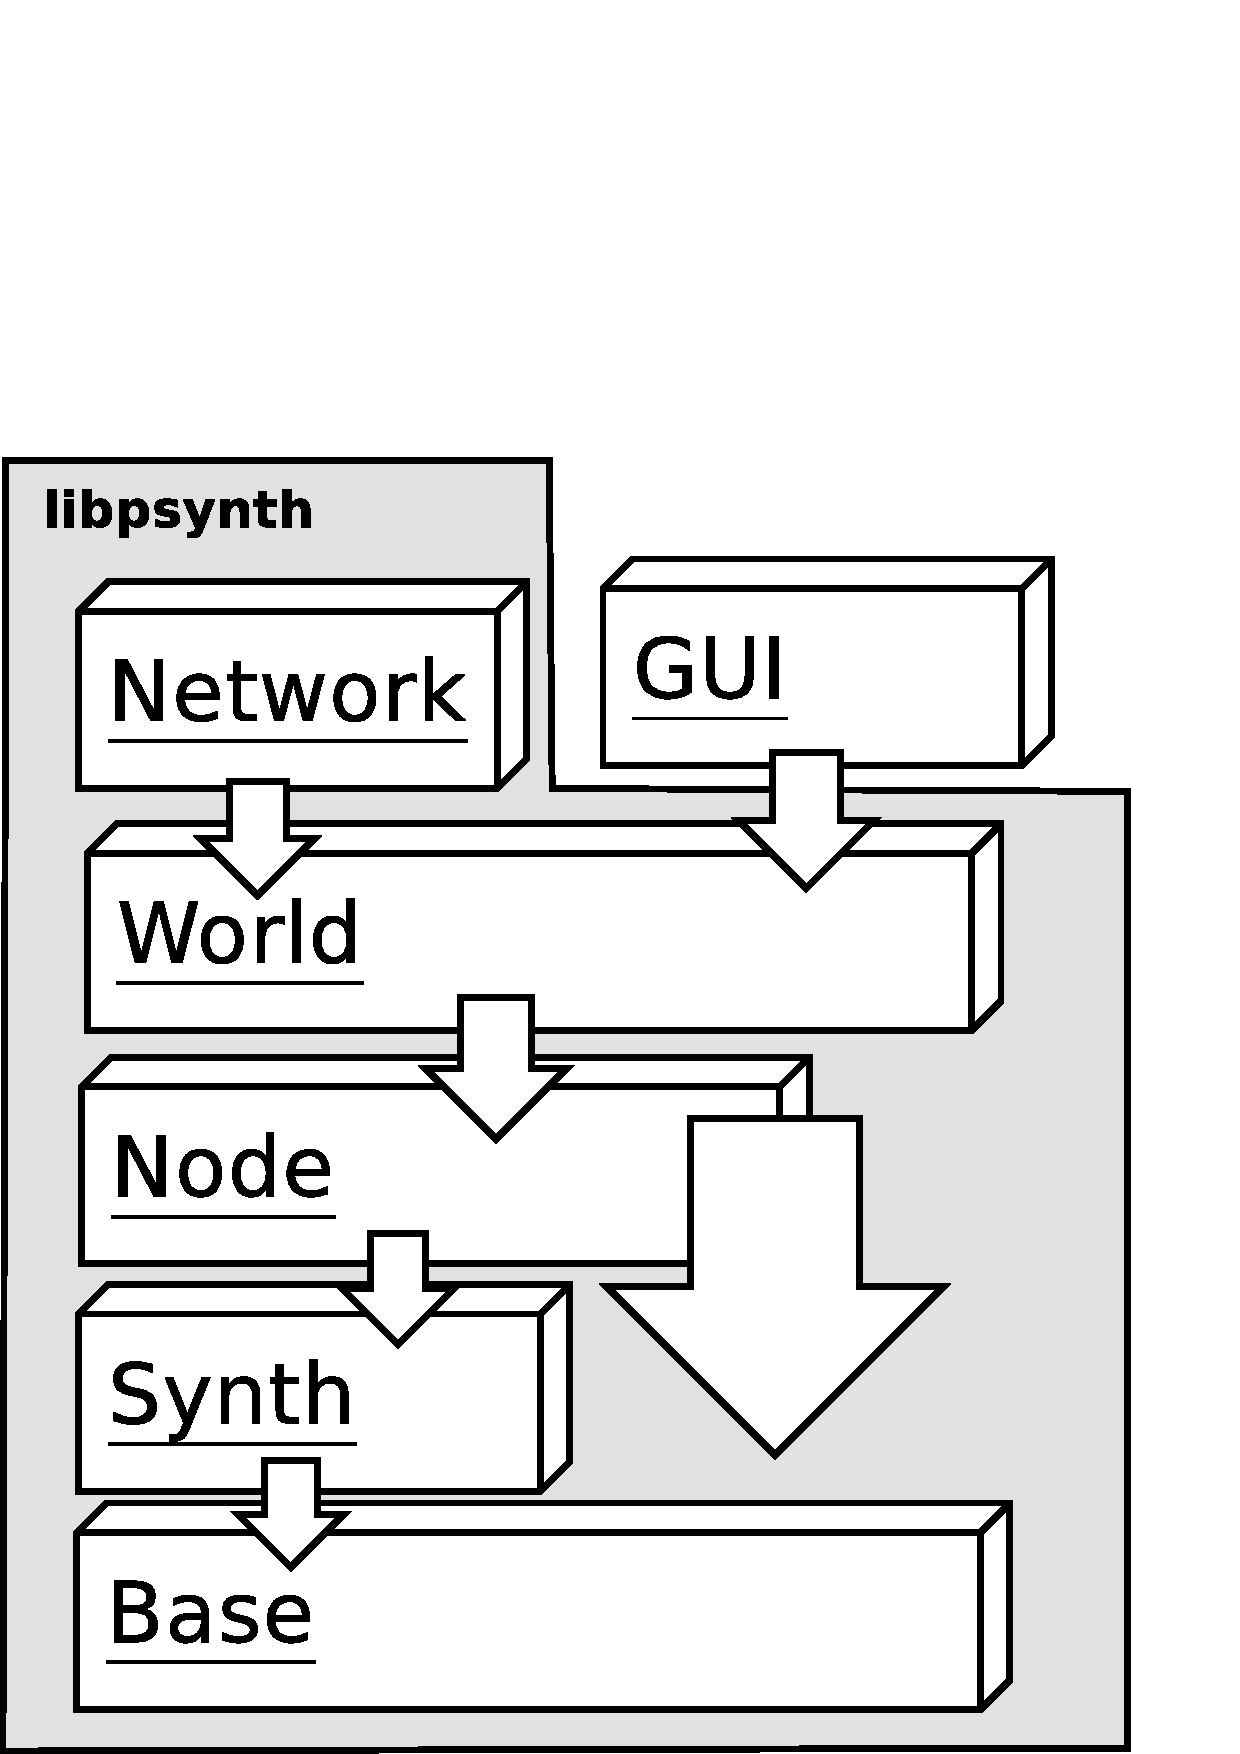
\includegraphics[width=.6\textwidth]{pic/layers.pdf}
\caption{The GNU Psychosynth layered architecture.}
\label{fig:layers}
\end{figure}

\subsubsection{The \texttt{base} layer}

The base layer\index{base (layer)} includes basic facilities that may
be reusable in any other part of the application. Some of the most
relevant examples are:

\begin{description}
\item[Configuration persistence] Classes for representing program
  settings in a hierarchical manner. This configuration system can use
  interchangeable backends and has an observable
  interface.\footnote{We use quite often the term \emph{observable
      interface} which is rare in the literature. By this, we mean
    that it provides signals, listeners or other event mechanisms,
    instances of the \emph{observer} design
    pattern\cite{gamma95design}.}

  In fact, we do not recommend using this module in the core of the
  intermediate layers of the library because it can cause unexpected
  coupling. Maybe in the future it will be moved to the thin
  \emph{app} module, but it is kept here for historical reasons.

\item[Implementation of design patterns] While the term \emph{design
    pattern}\index{design pattern} means reusable design structure,
  not reusable code, language abstractions can make them implementable
  generically in some cases. Andrei Alexandrescu proves this point for
  C++ in \cite{alexandrescu01modern}. This layer provides design
  pattern generic implementations inspired by Alexandrescu's
  approach. Some of the included facilities are implement
  \emph{observer}, \emph{singleton} and \emph{composite}.

\item[Command line argument parsing]\index{command line arguments}
  While we have considered moving to Boost's Program Options
  library\footnote{\url{http://www.boost.org/doc/libs/release/doc/html/program_options.html}},
  our own implementation have different trade-offs and is rather
  extensible.

\item[Logging system]\index{logging} A hierarchical and multi backend
  logging system for registering messages from other modules. It
  should be used instead of direct output to \texttt{std::cout/cerr}
  in all the code.

\item[File management tools] That ease the task of finding resources
  in the hard-drive and can cache results.
\end{description}

Some other minor classes and tools are excluded from this list. During
the development of the project we will drop in this layer classes that
feel interesting at any abstraction level.

\subsubsection{The \texttt{synth} layer}

\index{synth (layer)}This layer contains classes for the \emph{static}
construction of synthesisers and sound processing. The audio input and
output facilities are considered to be in this layer, and as well
audio processing data structures,--- like ring buffers, multi channel
buffersm, etc. --- basic implementations of filters, oscillators and
audio scalers.

By static, we mean that this code does not provide any dynamic routing
facilities, instead, the programmer is in charge to assign buffers and
call the processing elements manually.

Requisites \ref{req:iter1-begin} to \ref{req:iter1-end} should be
implemented here. Non functional requisites \ref{req:iter1-begin2} to
\ref{req:iter1-end2} are specially relevant in this layer too. Indeed,
this layer should be divided in three parts: the sound representation
library, the IO classes and the synthesis algorithms.

\subsubsection{The \texttt{graph} layer}

\begin{figure}[h]
\centering
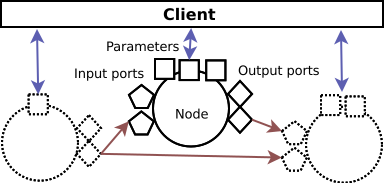
\includegraphics[width=.8\textwidth]{pic/node.pdf}
\caption[Representation of the node graph as in Psychosynth
0.1.7]{Representation of the node graph as in Psychosynth 0.1.7. Input
ports are represented as pentagons, output ports as rombus and
parameters as squares.}
\label{fig:node}
\end{figure}

This layer provides the facilities for the \emph{dynamic} construction
of synthesisers. It includes the mechanisms for describing and
executing the modular synthesis graph with the signal flow and so
on. Figure \ref{fig:node} represents the main concepts behind the
current design. Ports are considered as ``signal ports'' using the
terminology in requirement \ref{req:porttype} --- ``control ports''
are similar to ``parameters'', but parameters are not a precise model
of ``control ports'' as they can not be routed and are intended for
communication between the client user interface code and the audio
thread state. The communication system used to propagate values
between the audio processing thread and the client thread is
represented in figure \ref{fig:thread}. Values are copied to and from
an intermediate channel between the audio processing blocks.


\begin{figure}[h]
\centering
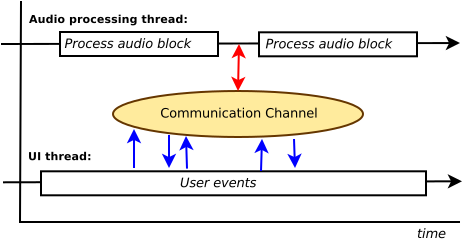
\includegraphics[width=.8\textwidth]{pic/thread.pdf}
\caption{Communication between the audio and user interface thread as
  in Psychosynth 0.1.7}
\label{fig:thread}
\end{figure}

Requisites \ref{req:iter2-begin} to \ref{req:iter2-end} should be
implemented in this layer. A heavy redesign of its API and many of its
internal implementation is to be expected for that to be
accomplished.

\subsubsection{The \texttt{world} layer and the Model View Controller
  architecture}

This layer simplifies the interface exposed to the previous layer and
makes it \emph{observable}\index{observer (design pattern)}. This is
fundamental for the Model View Controller that the system implements.
Figure \ref{fig:mvc} represents this architectural style. On the
following, we can refer to this observable interface abstracting the
synthesis engine as \emph{the model}\index{model (MVC)}.

\begin{figure}[h!] \centering
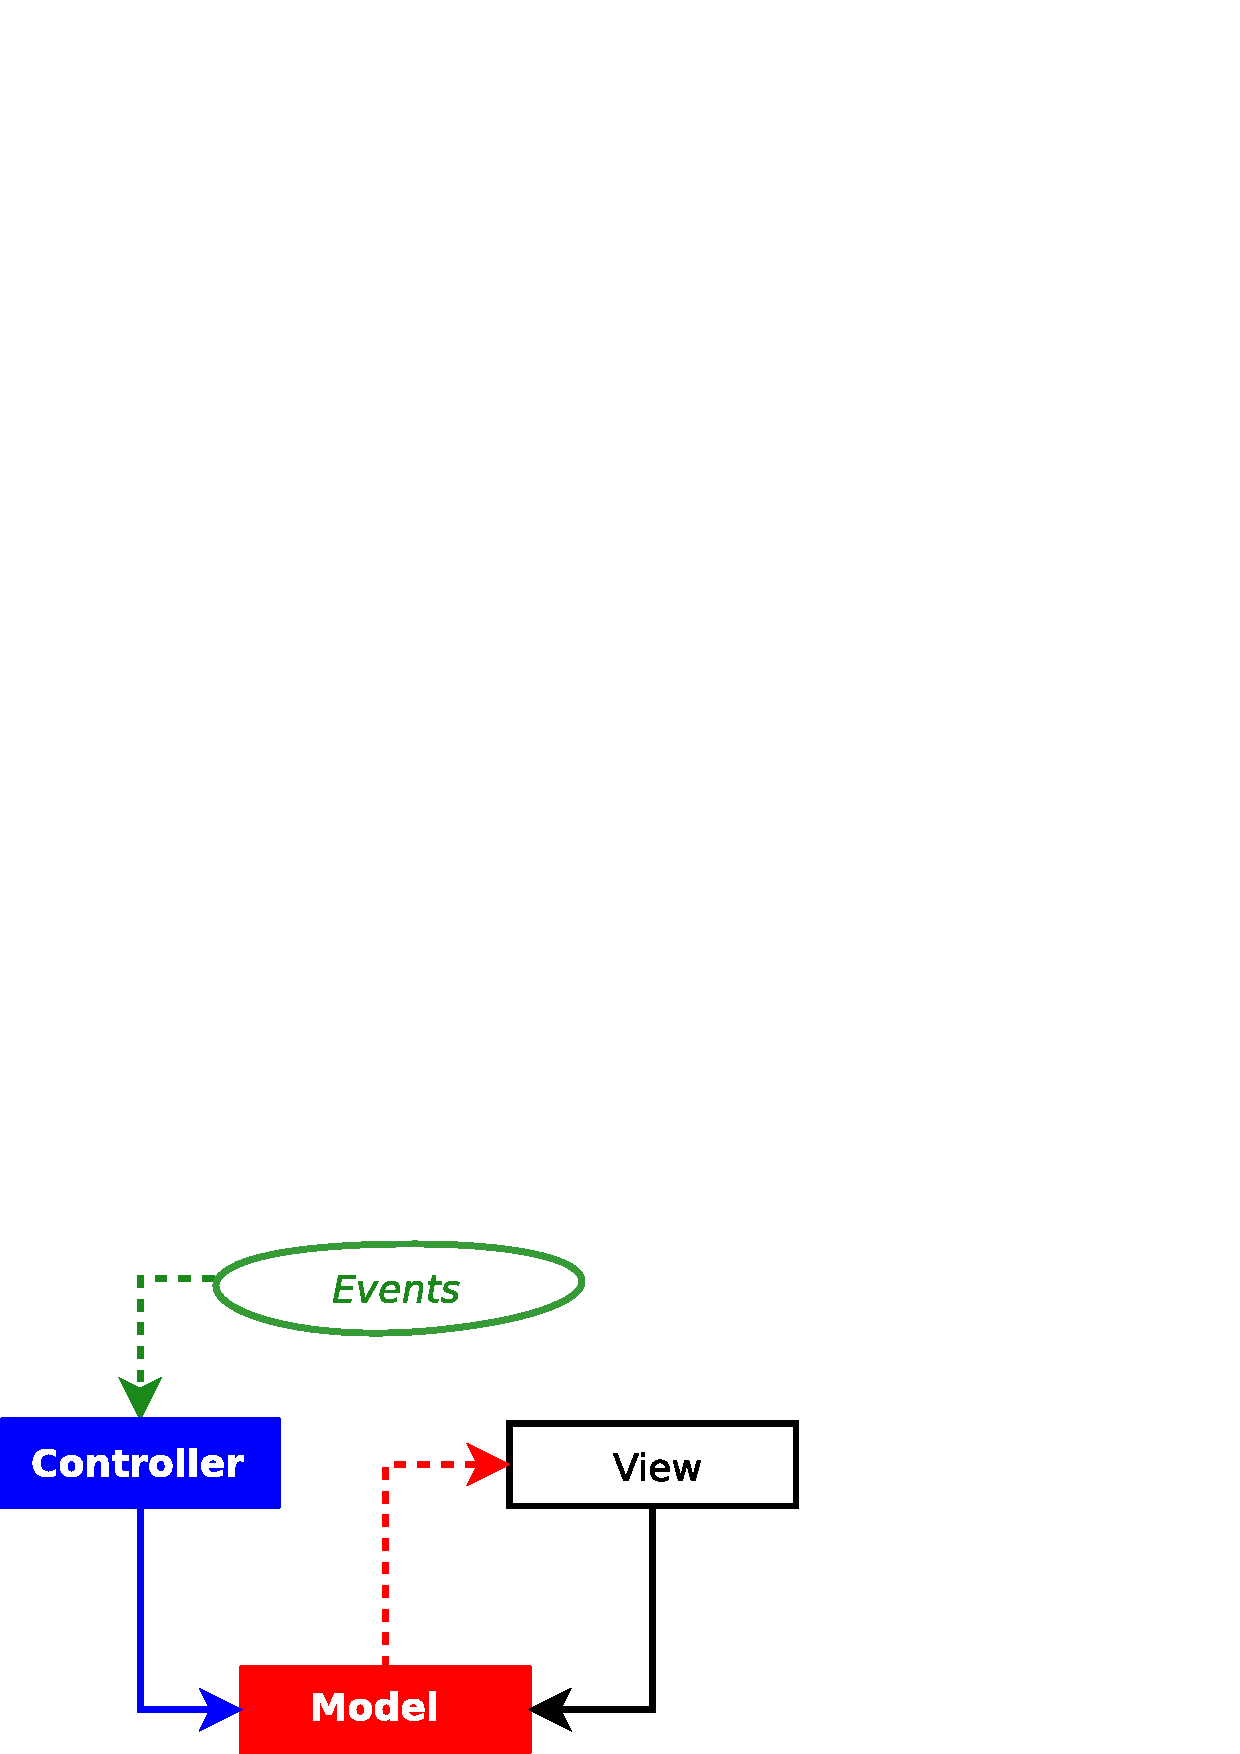
\includegraphics[width=.7\textwidth]{pic/mvc.pdf}

\caption[The MVC architectural style]{The Model View Controller
  arquitectural style. Dashed arrows represent indirect invocation
  ---i.e. via the \emph{observer} design pattern--- and normal lines
  represent normal method calls and data access.}
\label{fig:mvc}
\end{figure}

Several views\index{view (MVC)} can coexist independently --- for
example, a GUI user interface and a web client ---, that get updated
whenever a value has changed in the model. They register themselves on
the model at the beginning and then become passive entities that get
called by the model. The model changes when controllers invokes
methods on it, several controllers\index{controller (MVC)} can
coexists too. Usually, models and views come in pairs. For example, a
GUI view has an associated controller that triggers the manipulation
of the model in the eventuality of certain user actions like clicking
a button; in this case the representation (the buttons) and the action
(clicking it) are strongly related, but this is not necessarily true
in other situations.

This layer also abstracts the graph interconnection mechanism using
the \emph{strategy} design pattern\index{strategy (design
  pattern)}. Concretely, dynamic patching is implemented here and the
interface exposed in this layer hides the manual node interconnection
mechanisms but provides observability for topological changes.

This layer should implement requisite \ref{req:views}. 

\subsubsection{The application framework layer and some built-in views
  and controllers}

There is a thin layer, instance of the \emph{facade}
pattern\index{facade (design pattern)}, called \texttt{app}. It was
hidden for simiplicity in figure \ref{fig:layers} representing the
layered architecture. It sits on top of the \texttt{world} layer and
is in charge of initialising the \emph{world}, defines a configuration
tree using the facilities in the \texttt{base} layer, and setups the
machinery using the observability of the configuration system to keep
coherence between the user preferences and the status of the synthesis
model --- for example, if the ``\texttt{psynth.output}'' setting is
changed, it automatically creates the appropriate output object
instance, sets its values and substitutes the output node in the
synthesis graph. This layer also sets up the command line argument
parsing and installs some common audio setting arguments in the
parser. This layer is where Psychosynth becomes a
framework\index{framework} at its most pure level, as it offers a
\texttt{psynth\_app} class whose \texttt{run} method should be the
only call in the program \texttt{main}. This in turn delegates the
heavy work to user code that is hooked as method overrides of that
same class.

Orthogonal to this layer, and also sitting on top of the
\texttt{world} layer, the networking\index{networking} layer offers a
set of views and controllers\footnote{A primitive implementation of
  such at this stage of the development.}  that can be used to create
the shared environment described in requirement \ref{req:sharedenv}
--- thus enabling collaborative performances. This is an example of
the value of the MVC architecture: because views and controllers are
orthogonal, the user interface does not need to know about the
presence of this component to function properly. One could develop a
new experimental and cool UI and it would automagically be optionally
able to work with third party clients over the network, even
potentially using a different user interface.

In its current version, on top of all this, there is the code of the
3D user interface and some small and simple command line tools
intended to be used as GUI-less network capable clients and
servers. But all this code is not part of the framework. Instead, the
framework remain user interface agnostic, so we will not further
describe the UI code as it falls outside the scope of this project.

\section{Project planning and methodology}

\subsection{Rationale --- A critique on software engineering}

\index{software engeneering}Choosing a well known software engineering
process is considered one of the first steps to be taken in a final
master's thesis project. In our school we study with most detail the
Waterfall Model\index{waterfall model} \cite{benington87production}
and the Rational Unified Process\index{RUP, rational unified process}
\cite{kruchten03rup}.

Those development processes propose a fordist software production
model, targeted at huge development teams and the development of
stable code bases in non-experimental, well defined, fields. Many of
their proponents state that software engineering is like any other
engineering where creative analysis and design is only the first step
--- thus they believe programming is analogous to construction.
Fowler makes a great point \cite{fowler01design} criticising this
argument, as he says, the construction is done by the compiler and
people involved in programming are actually doing an intellectual and
creative work too --- in computing, any systematic task can and must
be automated indeed. The $programming=construction$ metaphor is
alienating for the programmer, who is completely excluded from the
task of criticising and improving the software design, and thus this
metaphor often leads, in the end, to bad software.

Moreover, these fordist development models take risk control and
client requirements satisfaction as most important factors. Because we
are in an academic environment, there are two more important factors:
the pedagogical value of the project --- this is, that the student
involved takes the risk of exploring the unknown by himself --- and
the research value --- this is, that the student involved takes the
risk of exploring the unknown by humanity.

Of course, this is neither a pure research project, so we can not
completely substitute a software development process by the scientific
method. But we can choose a more dynamic methodology that includes
\emph{falsification} in one way or the other. \emph{Agile}
methodologies\footnote{\url{http://agilemanifesto.org/}} propose many
alternatives that could be valid for a master thesis project.

Still, these methodologies are, we believe, inadequate for this
concrete project. The main reason is that this project is developed by
only one person. Agile methodologies put most emphasis on the
developer communication methods and collective decision making, so
they are often inadequate and too constraining and time consuming for
an unipersonal team, providing no additional value.  The Personal
Software Proccess \cite{watts96psp} proposes a methodology that is
specially targeted at personal software developed by engineering
students. Sadly, we are not very familiar with it --- and do not have
enough time to make that happen within the time constraints of the
project --- and it seems too be to specific and time consuming in its
time tracking proposal.

Because we still believe that some rational planning and methodology
is needed, we propose in the following a defined but unconstrained
methodology that is specially tailored for our circumstances,
capturing the most common elements in other software processes.

\subsection{An iterative development model}

Because of the size and complexity of the project, we should not
consider developing it all at once. Moreover, the layered architecture
of the starting code base and the variety of requirements that we want
to satisfy favour an iterative development.

Consequently, we want to split the development in iterations. Each
iteration is composed by the following phases: \emph{design},
\emph{implementation}, \emph{verification} and
\emph{integration}. Each iteration shall be assigned a set of
requirements from the specification in section \ref{sec:requirements}
that are to be satisfied after the successful accomplishment of that
iteration.

\subsubsection{The design phase}

\index{design}In the design phase we shall define the API that we
would like the current subsystem to have. Because we are developing a
library and framework with a public interface, the design phase is
specially relevant shall be done with care.

We do not enforce a particular method for documenting the design as
different programming paradigms favour different documentation
means. For example, in the first iteration we will develop a library
heavily based on metaprogramming, where UML does not fit very
naturally. Still, the documentation should include rationale
explaining why the design decision lead to the satisfaction of the
requirements assigned to that iteration. Also, it may be found that a
requirement may be impossible to satisfy on the current iteration or
that this requirement is to be better integrated in some other
iteration. The developer is free to reassign that requisite for later
iteration properly documenting this as a post-analysis plan fix.

What we do enforce is that all the API is documented with Doxygen for
the sake of completeness of the reference manual.

\subsubsection{The implementation phase}

\index{implementation}During the implementation phase the code
implementing the design should be written. It is possible and even
sometimes recommended to modify the design during this phase as
inconsistencies and fundamental problems are found. Sometimes, this
may even start as soon as design, specially when it is unclear the
properties that such API should have and some ``exploratory
programming'' is needed. This fact may or many not be documented in
the design document --- even though an API may be designed through an
inductive empirical process, a deductive rational description may be
more useful for its clear understanding indeed.

We are keen on Test Driven Development\index{TDD, test driven
  development} \cite{beck02tdd}. This methodology suggests that unit
tests should be written before the actual implementation for the
tested interface is written at all. Instead, a mock implementation is
to be provided. Once the tests compile --- and fail --- implementation
is started concentrating on making the tests pass. Once the tests do
pass, the code and internal design is improved via
\emph{refactoring}\index{refactoring}. We will not follow this
methodology dogmatically --- specially when exploratory programming is
required --- but we suggest to follow it whenever possible. Thus, we
can consider than the verification phase and implementation phase are,
or at least should be, overlapped.

\subsubsection{The verification phase}

\index{verification}In the verification phase we perform \emph{unit
  tests} on the most important parts of the system. No iteration
should be considered finished unless proper unit tests are written and
satisfied for its core components. For writing such tests the Boost
Unit Testing Framework should be used.

When some elements are considered relevant to performance
requirements, \emph{performance tests} should be included. While we do
not enforce a specific performance testing technique here, the
tests should be reproducible and automatable whenever possible.

\subsubsection{The integration phase}

\index{integration}When a subsystem is added and it is to replace an
existing subsystem in the project, the older code should be removed
and the layers on top must be modified such that they use the new
code. This might even be sometimes considered part of the
verification, as older tests working on the upper layers should be
checked to be working after the integration.

Informal integration tests should be done on the final user interface
to make sure that the properties of the older implementation are
preserved. Note that in most cases, we do not recommend to lose time
editing the old user interface such that the new features in the
framework are exposed to the user. Of course, that the new features
are usable is the final objective, but as it was justified in
\ref{sec:userinterface}, a completely new user interface will be
developed as part of a future project.

\subsubsection{Recursive decomposition of iterations}

In practice, some of the expected requirements to be satisfied may be
found orthogonal or maybe too big to be addressed at one. It is thus
allowed to recursively decompose an iteration in sub-iterations when a
first evaluation during the design phase suggests that.

\subsection{A project plan}

In the following we propose a project plan to accomplish the
requirements specified at the beginning of this chapter. As we stated
in the introductory chapter, this is a long-term project, and the
required effort to fulfil all the proposed objectives clearly exceeds
what a student can do in parallel to his normal studies\footnote{The
  student involved in this project, apart from being studying the
  normal courses for the 5th year in ``Ingeniería Informática'', he is
  also collaborating with the Computer Vision Group in the development
  of Moodle plug-ins (\url{http://nongnu.org/cvg-moodle/}), and has
  been hired by the Institute of Astrophysics of Andalucia to held a
  course in Advanced Python Programming in May
  (\url{http://sinusoid.es/python-avanzado/}). These time constraints
  must be taken into account in the project planning.}. \emph{Thus,
  only the two first iterations are to be developed in this mater's
  thesis}. This structure fits very well in the Spanish university
course structure; the first iteration shall be developed during the
first semester and the second iteration during the second and last
semester.

\subsubsection{First iteration: A metaprogramming based sound
  processing foundational library}

This iteration is here to deeply re-design the core data structures
using the latest techniques in C++. This requires special research and
performance requirements deeply rely on the success of this
iteration. 

Requirements \ref{req:iter1-begin} to \ref{req:iter1-end} and
\ref{req:iter1-begin2} to \ref{req:iter1-end2} should be satisfied for
its success.

Estimated time cost: 4 months.

\subsubsection{Second iteration: Redesign of the \texttt{node} layer
  for hierarchy and polyphony}

The \texttt{node} layer requires a redesign if we want to satisfy all
our purposes. Polyphony and hierarchy would be specially tricky to
implement directly on top of the current code base. A special
evaluation of how the new design interacts with the MVC architecture
and networking is required. The \texttt{world} layer may be affected
too. All the design changes should be implemented too.

Requirements \ref{req:iter2-begin} to \ref{req:iter2-end} should be
satisfied for its success. Requirement \ref{req:persistence} may be
optionally considered for its implementation in this iteration too.

Estimated time cost: 4 months.

\subsubsection{Third iteration: Dynamic loading of nodes}

In this iteration the plugin system is to be developed.

Requirements \ref{req:iter3-begin} to \ref{req:iter3-end} should be
satisfied for its success.

Estimated time cost: 3 months.

\subsubsection{Fourth iteration: Adding MIDI and synchronisation}

Synchronisation and MIDI support is one of the most important
features and it is also one of the features we know the least about,
thus, we should put special care on research and design. This will
affect the node and world layers mostly.

Requirements \ref{req:iter4-begin} to \ref{req:iter4-end} should be
satisfied for its success.

Estimated time cost: 5 months.

\subsubsection{Post mortem analysis}

After the conclusion of all the previous iterations, we should write a
conclusive report and evaluation of its success. Also, we should
prepare a final presentation for its evaluation.

\begin{mynote}[Structure of the rest of the documment]
  The rest of the documment is devoted for documenting the modules
  developed in the iterations that are expected to be developed within
  this master's thesis. Chapter \ref{sec:03-meta} describes the first
  iteration involving the new sound system. Chapter \ref{sec:04-graph}
  explains the new graph layer as developed in the second
  iteration. Finally, chapter \ref{sec:05-conclusion} recapitulates
  and will provide some sort of post-mortem analysis --- of these two
  iterations --- also preparing the ground for the future development
  of the project.
\end{mynote}

%%% Local Variables: 
%%% mode: latex
%%% TeX-master: "00-main"
%%% End: 


\chapter{A generic sound processing library}

\epigraph{Numbers it is. All music when you come to think.  Two
  multiplied by two divided by half is twice one.  Vibrations: chords
  those are. One plus two plus six is seven. Do anything you like with
  figures juggling. Always find out this equal to that. Symmetry under
  a cemetery wall. He doesn’t see my mourning. Callous: all for his
  own gut. Musemathematics. And you think you’re listening to the
  etherial. But suppose you said it like: Martha, seven times nine
  minus $x$ is thirtyfive thousand.  Fall quite flat. It’s on account of
  the sounds it is.}{\emph{Ulysses}\\\textsc{James Joyce}}

\todo{Este capítulo en general necesita más dibujos.}

\section{Analysis}

Requirements \ref{req:iter1-begin} to \ref{req:iter1-end} and
\ref{req:iter1-begin2} to \ref{req:iter1-end2} refer to the second
layer of our system --- in a bottom-up approach. The most crucial
question here: how do we represent a sound in a computer? Then, a new
question arises: how do we get the sound to the speakers? The later
question has a trivial answer --- use whatever API your operating
system exposes for delivering sound to the soundcard --- but the first
question is still to be answered. Actually, the solution to this first
question mostly subsumes the issue of how to interface with these
external interfaces, thus, shall we debate it with care.

\subsection{Factors of sound representation}
\todo{Me he dado cuenta de que esta sección introduce muchas
  definiciones. ¿Tal vez utilizar un estilo más formal usando el
  paquete theorem para las definiciones ayudaría a usar el documento
  como referencia?}

A sound signal is a longitudinal wave of air in motion. We can
analogically record the \emph{proximal stimuli} --- i.e. the physical
stimuli leading to the subjective act of perception
\cite{goldstein01sensation} --- sound by measuring the successive
oscillating values of air pressure in the observer's point in
space. Note that an static air pressure value can not be perceived and
the sensation of sound is caused by the relative oscillation of this
measure. The \emph{amplitude} of this change is associated to our
perception of \emph{loudness}, the frequency of this oscillation
mostly logarithmically determines our perception of pitch. We phrased
this conditionally because these two variables are actually
interrelated and our actual subjective perception of loudness might
vary with pitch and otherwise \cite{fletcher37loudness}.

Most of the time, we represent the relative air pressure value as a
voltage, that varies at some range --- p.e. $[ -5, 5 ] V$. This is an
analogous signal that we have to discretise somehow in order to
manipulate it computationally.

\subsubsection{Temporal quantisation}

Temporal quantisation relates to how many times per second do we store
the current voltage or air pressure value. The value of the signal
between to equally spaced in time samples is unknown, but we can use
some interpolation method to \emph{upsample} a signal --- i.e. to
figure out what is between two samples. Most of the time we refer to
the \emph{sampling rate}, in hertz, as the frequency of the temporal
quantisation.

We know from \emph{Niquist-Shannon sampling theorem} that perfect
reconstruction of a signal is possible when the sampling frequency is
greater than twice the maximum frequency of the signal being sampled,
or equivalently, when the \emph{Nyquist frequency} (half the sample
rate) exceeds the highest frequency of the signal being
sampled. Because the hearing range in most human beings is 20 Hz--20
kHz, audio compact discs use a 44.1 kHz sampling rate. Other popular
rates in audio production are 48 kHz, 96 kHz and 192 kHz. Sampling
rates bellow 44.1 kHz are used also in old computer games that were
limited by the computing power and low bandwidth systems such as
telephone, where low cost and proper understanding of human speech is
more important than audio fidelity.

The sound representation mechanism itself does not vary with the
sampling rate, and thus supporting various rates depends more on the
implementation of the signal processing units and the overall
performance of the system, with the CPU being able to process so many
samples per second being the biggest constraint.

\subsubsection{Spatial quantisation}

Spatial quantisation determines how many possible values can a sample
take in our finite and discrete scale. In a computer system, this is
determined by the size in bits of the underlying type used to store
the samples. An audio CD uses a \emph{bitdepth} of 16 bit with samples
that can take $65.536$ possible values while professional audio uses 24
bit or 32 bit samples. We can even see systems using 64 bit samples
during the processing to avoid accumulative rounding problems due to
heavy arithmetic. The \emph{dynamic range} of a signal with $Q$-bits
quantisation is:
\begin{equation}
  \mathrm{DR_{ADC}} = 20 \times \log_{10}(2^Q) = (6.02 \cdot Q)\, \mathrm{dB}
\end{equation}
The maximum \emph{signal-to-noise} ratio for such a system is:
\begin{equation}
  \mathrm{SNR_{ADC}} =  \left (1.76 + 6.02 \cdot Q \right )\ \mathrm{dB}
\end{equation}

Most analog systems are said to have a dynamic range of around 80 dB
\cite{fries05digital}. Digital audio CD have a theoretical
dynamic range of 96 db --- actual value is around 90 db due to
processing. Human hearing pain level is at 135 db but actually
prolonged exposure to such loud sound can cause damage. A loud rock
concert is around 120 dB and a classical music performance is at
110 db \cite{ludwig09music}, thus requiring bitdepth of at least 24
bit (theoretical dynamic range of 144 dB) for perfect fidelity.

There are some other aspects related to representation of samples in a
computer, such as the \emph{signedness} of the underlying type. Signed
types are usually considered more convenient for audio signals as 0
can be easily recognised as the still no-sound value simplifying
computations. Another important factor is whether we use \emph{fixed
  point} or \emph{floating point} arithmetic. While fixed point is
used in low-cost DSP hardware, floating point is the most common
representation in current audio software as nowadays processors are
optimised for SIMD\footnote{Single Instruction Multimple Data, as
  supported by MMX, 3D Now! and SSE extensions in Intel and AMD chips}
floating point arithmetic. Moreover, the algorithms implementation is
much harder to encode because products produce greater values and
there are many ways on how to account the carry.  Actually, even while
the actual bitdepth (the bit for the mantissa) of a 32 bit floating
point is the same of a 24 bit fixed point, then a 32 bit fixed point
will have a quite lower \emph{quantization error}, but the dynamic
range and SNR of a floating point is much higher because the
values are spaced logarithmically over a huge range
\cite{smith02dsp}. Another factor is the \emph{endianess} of fixed
point values but is relevant only when interfacing with file formats
and output devices.

\subsubsection{Channel space}

Because our hearing system is dicotomically symmetric, audio
engineers discovered that much better fidelity can be achieved by
reproducing the sound with some differences from two separate
loudspeakers. This is the well-known \emph{stereophonic} sound,
commonly named just \emph{stereo}.

For representing such a signal, two different streams of information
are needed for the left and right channels. Moreover, nowdays
\emph{quadraphonic}, and \emph{surround} sound with varying numbers of
channels up to 20.2 are used in different systems.

We call \emph{channel space} to the set of semantic channels we use in
some sort of audio representation --- p.e. stereo audio has channel
space with $left$ and $right$ elements. We use the term
\emph{frame} to call a set of samples coincident in time, this is, the
samples of the various channels at a given time point. Thus, we will
use most of the time the more accurate term \emph{frame rate}.

This rises the problem on how to linearise the multi channel data. The
most common mechanism in domestic hardware is by \emph{interleaving}
the samples of different channels, this is, by storing the frames
sequentially. However, high-end hardware often accepts data in
non-interleaved form where the samples of each channel is stored in a
separate sequence. In this document, we borrow from the image
processing world the term \emph{planar} to refer to non-interleaved
data. Software doing a lot of processing of the audio signal often
chooses this representation as it is easier to scale to varying number
of channels and split the signal to do per-channel filtering. Figure
\ref{fig:interleaving} compares visually the interleaved and planar
formats.

\begin{figure}[h]
  \centering
  \subfloat[]{\includegraphics[width=2in]{pic/fmt-planar.png}}\;
  \subfloat[]{\includegraphics[width=3in]{pic/fmt-interleaved.png}}
  \caption{Multi-channal data in planar (a) and interleaved (b) form.}
  \label{fig:interleaving}
\end{figure}

Another issue is the order in which the data from different semantic
channels is stored. We call a \emph{channel layout} a bijection $L : C
\rightarrow \mathbb{Z}_{\|C\|}$, where $C$ is a given \emph{channel
  space}. For example, the mapping $\{ left
\mapsto 0, right \mapsto 1 \}$ is a common layout for stereo sound,
but $\{ left \mapsto 1, right \mapsto 0 \}$ is sometimes used too.

\subsection{Common solutions}

As we have already noticed, 32 bit floating point sound with planar
left-right layout the most common in software of our kind during
internal processing. As most of this software is written in C, a
simple \texttt{float**} does the job. This was, actually, the internal
representation used in GNU Psychosynth in versions prior to 0.2.0,
wrapped in the \texttt{audio\_buffer} class.

However, this design starts to wobble whenever one has to interface
with some other library or hardware using a different format. Thus,
the \texttt{audio\_buffer} class provided different
\texttt{interleave\_*} and \texttt{deinterleave\_*}, where the
asterisk can be substituted by different sample formats like
\texttt{s16} or \texttt{s32} (fixed point signed 16 bit and 32 bit
respectively). This is very inconvenient because, as we have seen
through this section, many orthogonal factor affect audio
representation inducing a combinatorial explosion of format conversion
functions. Take a look at the 64 different read and write functions in
the \texttt{pcm.c} file of the
LibSndfile\footnote{\url{http://www.mega-nerd.com/libsndfile/}}
library.

This is a maintenance hell, but using the common means for abstracting
orthogonal behaviour variability, i.e. dynamic polymorphism, is simply
not an option in any audio software which supports real-time operation.

\subsection{A generic approach: Boost.GIL}

However, there is a piece of software that proved that this issue can be
solved in C++ using static polymorphism. This is the Generic
Image Library\footnote{http://stlab.adobe.com/gil} which was developed
by Ludovic Cortés et. Al inside Adobe Software Technology Lab that was
later include inside the Boost library distribution.

While sound and image manipulation are quite different, specially from
the psycho-perceptive point of view, they are both a signal processing
problem and thus share a lot in the representational issue. By
realising of a proper conceptual mapping between both worlds (table
\ref{tab:gilmap}), most of the library design and even quite a lot of
code of Boost.GIL can be reused to build a unique state-of-the-art
sound processing library that addresses the aforementioned issues in
an orthogonal generic manner while maintaining near-optimal
performance.

\begin{table}[h]
  \centering
  \begin{tabular}{c|c}
    Boost.GIL & Psynth.Sound \\ \hline\hline
    Channel   & Sample \\
    Color     & Channel \\
    Color Space & Channel Space \\
    Color Layout & Channel Layout \\
    Pixel & Frame \\
    View & Range \\
    Image & Buffer
  \end{tabular}
  \caption{Terminology map from \texttt{boost::gil} to \texttt{psynth::sound}}
  \label{tab:gilmap}
\end{table}

An \emph{image} is bidimensional matrix of \emph{pixels}, that capture
the properties of light electromagnetic waveform at those discrete
points. Each pixel, however, is decomposed in several \emph{colors}
that, for example, capture the intensity in the red, green and blue
sensors of a CCD camera. As there are different ways of decomposing an
audio frame (p.e, stereo, surround, etc.), there are different ways of
decomposing a pixel into several values, known as the \emph{color
  space} (p.e, RGB, CMYK, YUV, etc.). Boost.GIL uses the term
\emph{channel} to name the individual value of one those color
components.

In our audio framework, a \emph{buffer} is unidimensional array of
\emph{frames} that represent a sound or part of a sound --- sound is
continuous and thus we usually process it in chunks. The reader might
note that the the data in a buffer being arranged along the
\emph{time} dimension while the dimensions of an image represent
\emph{physical space} makes these entities completely different from
the processing point of view. However, they share most representation
problems, with sound representation being actually a sub-problem of
image representation, as we have one dimension less. The samples in a
series of audio frames can be stored in an interleaved or planar
fashion as happens with the channels of a pixel. Also, both channels
and samples can vary in signedness, fixed/floating point, bitdepth,
etc.

Those already familiar with Boost.GIL can thus already understand
easily our Psynth.Sound module design and implementation that we are
to describe in the following section.

\section{Design}

\subsection{Core techniques}

The Boost.GIL and thus the Psynth.Sound modules design makes heavy use
of static polymorphism and generic programming via C++ templates to
achieve generality without runtime overhead. We are going to introduce
advanced techniques used in generic programming for the reader
unfamiliar with this programming paradigm.

\subsubsection{Concepts}
\label{sec:concepts}.

\emph{Concepts} \cite{jarvi10concept} are to generic programming what
\emph{interfaces} --- pure abstract classes in C++ --- are to object
oriented programming: they specify the requirements on some
type. However there, are few substantial differences. (1) While
interfaces can only specify the method signatures of its instances, a
concept can specify most syntactic constraints on a type, like the
existence of free functions, operators, nested types, etc. (2) While
dispatching through interfaces requires, at least, a dereference,
addition and function call \cite{driesen96direct}, when using concepts
the concrete function to be executed can be determined and even
inlined at compile-time. (3) One can not declare that a type satisfies
an interface separately from the type definition, but one can say that
a type models a concept at any point of the program. (4) Thus, no
primitive type defines any virtual interface, but one can turn any
primitive type into an instance of any concept via a
\texttt{concept\_map}. (5) Actually, the syntactic properties defined
by a concept its models may differ, but they are matched via the
\texttt{concept\_map}. In fact, C++ concepts are more similar to
Haskell \emph{type classes}, with \texttt{instace} doing the job of
\texttt{concept\_map} \cite{bernardy08comparison}.

Concepts are an extension to the template mechanism to add type
checking for it. In fact, checking and dispatching on requirements can
be achieved with techniques like SFINAE (Substitution Failure Is Not
an Error) \cite{vandervoorde08templates}. Property (5) of our concepts
can be simulated with \emph{traits} \cite{c++traits}. However, both
compiler errors and the code using templates without concepts is
usually much more unreadable.

The proposal of adding concepts to the C++ language was rejected last
year by the standardisation committee and thus we can not use them in
our code. However, Boost.GIL is very influeced by Alexander Stepanov's
deductive approach to computer programming using generic programming
and modeling with concepts, that he elegantly describes in his
master-piece ``Elements of Programming''
\cite{stepanov09elements}. Actually Stepanov worked several years in
Adobe where he held a course ``Foundations of Programming'' based on
his book. Thus, the \emph{modeling} of the library extensively uses
concepts. Its implementation uses a limited form of concept checking
via the Boost.ConceptCheck\footnote{
  Boost.ConceptCheck: \url{http://www.boost.org/doc/libs/release/libs/concept_check/concept_check.htm}}
\cite{siek00concept} library, however, enabling this library in
release mode can affect performance and its syntax is quite more
cumbersome than the concepts in the C++ standard proposal. For
consistency with the Boost.GIL documentation we will use the concept
syntax proposed in the proposal N2081 to the standardisation committee
\cite{gregor06concept}.

The following example defines a concept that is satisfied by every
type that has an \texttt{operator<}:

\begin{lstlisting}
concept LessThanComparable<typename T> {
  bool operator< (T, T);
};
\end{lstlisting}

This allows us to write a generic function that depends on the
existence of a less-than comparator for the parametrised type:

\begin{lstlisting}
template<LessThanComparable T>
const T& min (const T& x, const T& y) {
  return x < y? x : y;
}
\end{lstlisting}

An alternative syntax for specifying that \texttt{T} must satisify the
\texttt{LessThanComparable} concept is the \texttt{where} clause:

\begin{lstlisting}
template<typename T>
    where LessThanComparable<T>
const T& min (const T& x, const T& y) ...
\end{lstlisting}

In fact, this is the only valid syntax when the concept affects
multiple types. Also, the \texttt{where} clause can be used inside
concept definitions to provide specialisation.

Specifying that a type models a concept is done with the
\texttt{concept\_map} device. If the type naturally models the
concept, we can just use:

\begin{lstlisting}
concept_map LessThanComparable<int> {}
\end{lstlisting}

Note that these trivial concept mappings can be avoided by using the
\texttt{auto} keyword in front of the \texttt{concept} keyword in the
concept definition. However, it might happen that a type requires some
wrapping to satisfy the concept. We can do this in the concept map
definition itself.

\begin{lstlisting}
concept_map LessThanComparable<char*> {
  bool operator< (char* a, char* b) {
    return strcmp (a, b) < 0;
  }
}
\end{lstlisting}

Note that this last piece of code is an example of a bad usage of
concept maps, as this specialises the mapping for pointers changing
the expected semantics.

This should suffice as an introduction to concepts in order to
understand the concept definitions that we will later show when
modelling our system. A more detailed view can be read in the cited
bibliography, with \cite{jarvi10concept} being the most updated and
useful from a programmer point of view.

\subsubsection{Metaprogramming}

The C++ template system is Turing complete
\cite{veldhuizen03templates}, thus it can be used to perform any
computation at \emph{compile time}. This was first noted in 1994 by
Erwin Unruh who, in the middle of a C++ standardisation committee,
wrote a template meta-program that outputted the first $N$ prime
numbers on the console using compiler errors \cite{unruh94prime}. Even
though this might seem just a crazy puzzle game, it can be used in
practise and actually new Boost libraries use it extensively. A very
gentle introduction to template metaprogramming can be found in
\cite{alexandrescu01modern}, where Alexandrescu uses them to
instantiate design patterns as generic C++ libraries. A deeper
reference is Abraham's \cite{abrahams04meta}, which focuses on the
Boost Metaprogramming Library\footnote{The Boost.MPL:
  www.boost.org/doc/libs/release/libs/mpl} and introduces the usage of
metaprogramming for building Embedded Domain Specific Languages (EDSL)
in C++. This Boost.MPL, providing reusable meta data structures and
algorithms, is the de-facto standard library for template
metaprogramming\footnote{It is often called ``the STL of template
  metaprogramming''.} and we will use it in our implementation.

Template metaprogramming is possible thanks to \emph{partial template
  specialisation}, that allows giving an alternate definition for a
pattern matched subset of its possible parameter values. A
\emph{metafunction} is thus just a template \texttt{class} or
\texttt{struct} with a public member that holds the result of the
function. It is up to the programmer to choose the naming convention
for the result members of the metafunctions, in the following, we will
use Abraham's style calling \texttt{type} for result values that are a
type, and \texttt{value} for integral values. Listing \ref{lst:fib}
illustrates how can we write and use a metafunction for computing the
$n$-th Fibonacci number.

\begin{lstlisting}[float=h!, 
  caption=Metaprogram for computing the Nth Fibonacci number,
  label=lst:fib]
template <int N>
struct fib {
  enum { 
    value = fib<N-1>::value + fib<N-2>::value; 
  };
};

template <>
struct fib <0> {
  enum { value = 0 };
};

template <>
struct fib <1> {
  enum { value = 1 };
};

int main () {
  return fib<42>::value;
}  
\end{lstlisting}

The program returns the forty-second Fibonacci value. However, it will
take no time to execute, because the number is computed at compile
time. We use recursion to define the metafunction for the general case
and the specialise for the base cases.

If we consider the template system as a meta-language on its own, we
should describe its most outstanding semantic properties. It is a pure
functional programming language, because variables are immutable. It
is lexically scoped. It supports both lazy and strict evaluation,
depending on whether we choose to access the nested \texttt{type}
result name at call site or value usage type. When we look at the meta
type system, we find three meta types: types (which are duck-typed
records), integrals (e.g. \texttt{int}, \texttt{char}, \texttt{bool}
...) and meta-functions (i.e. templates).

The fact that records are duck typed but integrals and metafunctions
cause several inconveniences in practice, specially when dealing with
the later. For example, in the absence of template aliases, returning
a metafunction produced by another function requires defining a nested
struct that inherits from the actual synthesised value. Also, the
template signature should be specified on a template parameter
expecting a template.

In order to simplify our meta type system we shall wrap constants in a
type like on listing \ref{lst:integral_c}.

\begin{lstlisting}[float, 
  caption=Integral constant nullary metafunction  wrapper.,
  label=lst:integral_c]
template <typename T, T V>
struct integral_c
{
  BOOST_STATIC_CONSTANT(T, value = V);
  typedef integral_c<T, V> type;
};
\end{lstlisting}

There are a couple of issues regarding this definition worth
explaining. First, the \texttt{BOOST\_STATIC\_CONSTANT} macro is used
to define a constant. Internally, it will try to use \texttt{enum} or
any other mechanism available to actually define the constant such
that the compiler is not tempted to allocate static memory for the
constant. Second, the \texttt{typedef} referring to itself turns a
constant value into a self returning nullary meta-function. This can
be very convenient because, for example, it allows using
\emph{value}\texttt{::type::value} always on the value usage point,
allowing the caller or producer of the value to choose whether he
wants to evaluate the value lazily.

Because we just wrapped values into a type, we can simplify our
conventional definition of \emph{metafunction}: a meta-function is any
type --- template or not --- that has a nested type called
\texttt{type}.

Now we should also turn metafunctions into first class entities of the
meta-language. We just add a new level of indirection and define a
\emph{metafunction class} as a type with a nested template
metafunction called \texttt{apply}. The example in listing
\ref{lst:high_order_fib} also illustrates the metafunction forwarding
technique when defining the nested \texttt{apply} metafunction by
inheriting from \texttt{fib}.

\begin{lstlisting}[float, caption=Metafunction class for
  computing Fibonacci numbers. We suppose that the previous
  \texttt{fib} definition uses \texttt{integral\_c} to wrap its
  parameters and return types., label=lst:high_order_fib]
struct fib_class { 
   template <class N>
   struct apply : public fib<N> {};
};

int main ()
{
  return fib_class::apply<integral_c<int, 42>>::type::value;
}
\end{lstlisting}

Using this convention the MPL library defines many useful high order
metafunctions that take metafunction classes as input, like
\texttt{mpl::fold} and \texttt{mpl::transform}. Note that it is not
needed to define metafunction classes for all our metafunctions,
instead, we shall convert them when needed using the
\texttt{mpl::quote}\emph{N} functions and the \texttt{mpl::lambda}
facility.

\subsection{Core concepts}

We are now ready to understand the main design and implementation
techniques used in our generic library. Because the library is
\emph{generic}, in the sense of generic programming, most algorithms
and data structures are parametrised such that they can be
instantiated with any concrete type modelling some concepts as we
suggested in section \ref{sec:concepts}. Thus, traditional modelling
techniques like the Unified Modelling Language are not useful since
they are intended for object oriented design.

We are going to follow the following methodology for describing the
library. First, we will name a concept and give a brief description of
its purpose. Then, we will define the concept using the notation
described in section \ref{sec:concepts} and finally we will enumerate
and describe some models for such concept.

For brevity, we will omit basic concepts such as
\texttt{CopyConstructible}, \texttt{Regular}, \texttt{Metafunction},
etc. Their complete definition should be evident and an interested
reader can find most of them in \cite{stepanov09elements}.

\subsubsection{\texttt{ChannelSpaceConcept}}

A channel space is a sequence of whose elements channel tags (empty
types giving a name )

\begin{lstlisting}
concept ChannelSpaceConcept<MPLRandomAccessSequence Cs> 
{};
\end{lstlisting}

Some example models include \texttt{stereo\_space} or
\texttt{surround\_space}. An example on how a user of the library can
define his own channel space follows.

\begin{lstlisting}
struct left_channel {};
struct right_channel {};

typedef mpl::vector<left_channel, right_channel> stereo_space;
\end{lstlisting}

A related trivial concept is
\texttt{ChannelSpaceCompatibleConcept}. Two channel spaces are
compatible if they are the same. In fact, this leaks the underlying
MPL sequence type used in the channel space through the abstraction,
because spaces with the same set of semantic channels might be found
incompatible, but it suffices in practise.

\subsubsection{\texttt{SampleConcept}}

A \emph{sample} is the type we use to represent the amplitude of a
channel at certain point in time.

\begin{lstlisting}
concept SampleConcept<typename T> :
             EqualityComparable<T> {
    typename value_type      = T;
    // use sample_traits<T>::value_type to access it
    typename reference       = T&;
    // use sample_traits<T>::reference to access it
    typename pointer         = T*;
    // use sample_traits<T>::pointer to access it
    typename const_reference = const T&;
    // use sample_traits<T>::const_reference to access it
    typename const_pointer   = const T*;
    // use sample_traits<T>::const_pointer to access it
    static const bool is_mutable;
    // use sample_traits<T>::is_mutable to access it

    static T min_value(); 
    // use sample_traits<T>::min_value to access it
    static T zero_value(); 
    // use sample_traits<T>::zero_value to access it
    static T max_value(); 
    // use sample_traits<T>::min_value to access it
};
\end{lstlisting}

Built-in scalar types like \texttt{char}, \texttt{int} or
\texttt{float} model \texttt{SampleConcept} by default. 

The \texttt{scoped\_sample\_value<Type, Min, Max, Zero>} template
class models the concept whenever \texttt{Type} is a scalar type and
\texttt{Min}, \texttt{Zero} and \texttt{Max} satisfy:
\begin{equation}
Min < Zero < Max \land \forall x \in Type, x + Zero = x
\end{equation}
Note that, in order to avoid the limitation of floating point values
not being usable as template arguments, \texttt{Min}, \texttt{Zero}
and \texttt{Max} should be a type with a static method
\texttt{apply()} that returns the actual value. It should be used to
constraint the ``clipping thresholds'' of floating point types. For
example, the \texttt{bits32sf} model defined as:

\begin{lstlisting}
  scoped_sample<float,
                float_minus_one,
                float_zero,
                float_one>;
\end{lstlisting}

User defined types should specialise \texttt{sample\_traits} to map
the concept.

Related trivial concepts are \texttt{MutableSampleConcept} and
\texttt{SampleValueConcept} (a sample that is also \texttt{Regular}).

\subsubsection{\texttt{SampleConvertibleConcept}}

Because casting does not suffice in most cases, one should
override a \texttt{T sample\_convert (U)} function for \texttt{U} to
be convertible into \texttt{T}.

\begin{lstlisting}
concept SampleConvertibleConcept<SampleConcept SrcSample,
     SampleValueConcept DstSample> {
    DstSample sample_convert (const SrcSample&);
};
\end{lstlisting}

The library provides overrides for \texttt{sample\_convert} making
most supplied sample types being convertible too.

\subsubsection{\texttt{ChannelBaseConcept}}

A \emph{channel base} is a container of channel elements (such as
samples, sample references or sample pointers).

The most common use of channel base is in the implementation of a
frame, in which case the channel elements are sample values. The
channel base concept, however, can be used in other scenarios. For
example, a planar frame has samples that are not contiguous in
memory. Its reference is a proxy class that uses a channel base whose
elements are sample references. Its iterator uses a channel base whose
elements are sample iterators.

\begin{lstlisting}
concept ChannelBaseConcept<typename T> :
      CopyConstructible<T>, EqualityComparable<T>
{
    // a Psynth layout (the channel space and element permutation)
    typename layout;     
        
    // The type of K-th element
    template <int K> struct kth_element_type;
    where Metafunction<kth_element_type>;
    
    // The result of at_c
    template <int K> 
    struct kth_element_const_reference_type;
    where Metafunction<
            kth_element_const_reference_type>;        
    
    template <int K> 
    kth_element_const_reference_type<T,K>::type at_c(T);

    // Copy-constructible and equality comparable 
    // with other compatible channel bases
    template <ChannelBaseConcept T2> 
        where { ChannelBasesCompatibleConcept<T,T2> } 
        T::T(T2);
    template <ChannelBaseConcept T2> 
        where { ChannelBasesCompatibleConcept<T,T2> } 
        bool operator==(const T&, const T2&);
    template <ChannelBaseConcept T2> 
        where { ChannelBasesCompatibleConcept<T,T2> } 
        bool operator!=(const T&, const T2&);
};
\end{lstlisting}

A channel base must have an associated layout (which consists of a
channel space, as well as an ordering of the samples).  There are two
ways to index the elements of a channel base: A physical index
corresponds to the way they are ordered in memory, and a semantic
index corresponds to the way the elements are ordered in their channel
space.  For example, in the stereo channel space the elements are
ordered as \texttt{\{left\_channel, right\_channel\}}. For a channel
base with a RL-stereo layout, the first element in physical ordering
is the right element, whereas the first semantic element is the red
one.  Models of \texttt{ChannelBaseConcept} are required to provide
the \texttt{at\_c<K>(ChannelBase)} function, which allows for
accessing the elements based on their physical order. Psynth provides
a \texttt{semantic\_at\_c<K>(ChannelBase)} function (described
later) which can operate on any model of \texttt{ChannelBaseConcept}
and returns the corresponding semantic element.

The library provides an \texttt{homogeneous\_channel\_base} class that
models the concept.

\subsubsection{\texttt{...Concept}}

\subsection{Going dynamic}
\subsection{Input and Output module}
\subsection{Synthesis module}

\section{Validation}

\subsection{Unit testing}


\subsection{Performance}

\subsection{Integration}

The module was first developed separately from the main development
branch in a branch called \texttt{gil-import}. Once the previous tests
were passed, the former signal representation classes and I/O code was
removed from the code base. The upper layers --- mainly the
\texttt{graph} layer --- was adapted to use the new library. Note
that, given that we will mostly rewrite the \texttt{graph} layer in
the next iteration we tried to make minimal changes to get the project
compile and run properly again.

The system was then \emph{peer reviewed} by project collaborators,
mainly by the maintainer of the Ubuntu/Trinux packages Aleksander
Morgado\footnote{Aleksander Morgado's web blog:
  \url{http://sigquit.wordpress.com}}. After minor bugfixing, we
agreed to make a new Psychosynth 0.2.0 release that included the new
code described in this chapter and some other fixes and modifications
developed alongside.

The official changelog briefing for this release is included in note
\ref{note:changelog02}.

\begin{mynote}[Changelog of Psychosynth 0.2.0]
\label{note:changelog02}
\begin{itemize}
\item New audio processing and I/O subsystem based on template programming
for generic yet efficient sound signals.

\item The extreme latency when using ALSA bug seems to be fixed in
  some cases.

\item No longer depend on libvorbis, libsndfile can now handle ogg and flac
files too.

\item No longer depend on \texttt{libsigc++}, using \texttt{boost::signals}
  which, which is a bit slower but neglibe and this simplifies the
  dependencies.

\item The mouse wheel now scrolls in the object selector.

\item The object selector no longer lets mouse clicks pass through.  

\item Backwards reproducing a sample works a bit better now too.

\item Some new niceties in the framework base layer, including some
  experiments on applying the C3 class linearisation algorithm in raw
  C++.

\item C++0x features are being used in the code. For GCC, this means
  version 4.5 shall be used. We doubt it will compile with any other
  compiler (maybe latest VS), but users are welcomed to try and report.

\item For this same reason, Boost.Threads is no longer a dependency,
  we use STL threads instead.
\end{itemize}
\end{mynote}

\section{Conclusions}

In this iteration we developed a generic approach to representation
and input and output of audio data. We do not have any records of
any audio software using such paradigm in their code, so this
development have been exploratory and has a lot of value in its
novelty. This however delayed our development more than expected in
our original plan.

\subsection{Benefits and caveats}

The three main advantages in the new code are:
\begin{enumerate}
\item Code can be mostly abstracted from the audio format
  representation while retaining near optimal performance. Because
  generality allowed decoupling orthogonal concepts, each audio
  representation factor can be optimised and tuned for computational
  accuracy on its own, leading to higher quality code with lower
  maintenance cost as we avoid the combinatorial explosion that
  happens otherwise.

\item Algorithms correctly written with our generic facilities have a
  performance equivalent to the hand-written code. When a certain
  algorithm has not general interpretation or can not be efficiently
  implemented generally, the library still allows for the algorithm to
  be written with for a concrete or a constrained family of audio
  formats.

\item Because the signal format is encoded in the data type, we can
  either statically check that the data is in the correct format
  through our processing chain, or trivially enforce runtime checks
  when the format is unknown at compile time (via
  \texttt{dynamic\_buffer} and similar tools), leading to more secure
  code.
\end{enumerate}

Also, because a lot of learning have happened since the old code base
was written, the new code is better written and quite safer, making
use of exceptions and scope guards \cite{alexandrescu00gener}.

Even though we believe the benefits outweight the drawbacks, we have
to acknowledge the caveats of our new approach, the most relevant
being:

\begin{enumerate}
\item The new code uses advanced C++ programming techniques that many
  programmers find hard to understand. Thus, it might be harder for
  casual contributors to join the project in the future.

\item In the absence of real language support for concepts, template
  metaprograms leak their implementation in user code's compilation
  errors. This is so because, actually, by expanding the type
  instantiations in the compilation error, the compiler is actually
  showing a full backtrace of the metaprogram. This leads to cryptic
  error messages that often obfuscate the real source of the problem,
  discouraging novel developers.

\item Template metaprograms take longer to compile. However, proper
  usage of the new \texttt{extern template} facility should avoid
  redundantly instantiating templates in different translation units
  only to be discarded by the linker mostly solving this issue. Also,
  because the compiler generates different object code for each audio
  format, thoughtless use of the library can lead to code bloat and
  too large binary size.
\end{enumerate}

\subsection{Future work}

While the current status of the library is quite satisfactory for our
needs, there is still a lot of room for improvement that we will
postpone since they fall outside this project's scope. Nonetheless it
is worth enumerating them:

\subsubsection{Virtual and adapted iterators and ranges}

Boost.GIL included a ``locator adapter'' and ``virtual locator''
notions that allowed creating or modifying images lazily via a
function object. We discarded implementing them because they were
coupled to their \texttt{locator} concept which is specific to the
problem of image representation --- locators are in practice 2D
iterators. Moreover, they used the indexed position in the image as
the parameter to the function object that synthesised the
image. However, because audio is processed in chunks, the position in
the audio buffer is meaningless for the synthesis or filter function
--- instead, some stateful function object which includes a notion of
time position related to the frame rate is needed. Thus, many
unexplored design decisions should be taken, and the interactions with
other similar libraries like Boost.Iterator\footnote{The
  Boost.Iterator Library:
  \url{http://www.boost.org/doc/libs/release/libs/iterator}} and
Boost.Range\footnote{The Boost.Range Library:
  \url{http://www.boost.org/doc/libs/release/libs/range}} should be
carefully evaluated.

\subsubsection{Better arithmetic support}

The library includes some basic arithmetic support for samples. There
are few complications when developing full generic arithmetic support
for samples and frames. As Lubomir Bourdev, lead developer of
Boost.GIL, stated it in an email conversation with us:

\begin{quotation}
``Doing arithmetic operations is tricky for a number of reasons:

\begin{itemize}
\item What do you do on overflow? Clip, throw exception, allow out of
  range values?

\item What is the type to be used during conversion? Even if the
  source and destination have the same type, the operation might need
  to be done in another type and then cast back.

\item Certain arithmetic operations have no meaningful interpretation
  as far as color is concerned, such as multiplying one pixel by
  another. 
\end{itemize}

Because of issues like these we have not tackled the problem of
providing arithmetic operations, but we have provided generic
operations that can be done per channel or per pair of channels which
could be the basis for arithmetic operations.''
\end{quotation}

Nonetheless with time and effort the problem could be
approached making some compromises. Some of the issues Lubomir states
have different answers for sound processing, in fact, allowing out of
range values is the best answer for the first question given the fact
that sound amplitude is not naturally constrained and clipping is
introduced only by the DAC hardware or when moving from floating to a
fixed point representation. Maybe, not all those questions have to be
answered in order to improve the arithmetic support.

One of the main annoyances when writing a generic algorithm is using
the per sample \texttt{static\_*} algorithms. Using them we could
write a simple arithmetic layer for frames that would simplify the
user code. However, even though we do not have experimental data, we
believe this straightforward solution could introduce overhead. This
is because every \texttt{static\_*} unrolls one statement per
channel. Thus, a simple frame arithmetic expression would in fact
result into many sequence points that is yet to be tested whether
compilers can optimise properly.

This is not a dead end. Using the \emph{expressions templates}
\cite{veldhuizen95expression} technique and r-value references we can
perform transformations with the aid of metaprogramming such that
sequence points are not introduced by the arithmetic expression
itself. A expression template framework like Boost.Proto\footnote{The
  Boost Proto library:
  \url{http://www.boost.org/doc/libs/release/libs/proto}}
\cite{niebler07proto} could be of great help. Moreover, with careful
studying of the audio DSL's studied in section \ref{sec:dsl} and the
usage of these same techniques the scope of such effort could be
broadened to build a full sound synthesis and processing EDSL for C++.

\subsubsection{Submission to Boost}

In our conversations with Lubomir Bourdev he suggested submitting our
library for inclusion in the Boost package. However, there are few
issues that we should tackle before that:

\begin{enumerate}
\item A lot of code is algorithmically identical to that of Boost.GIL
  with changes only in terminology. A lot of work in properly
  abstracting such common parts should be made to avoid code
  repetition and doubled maintenance effort inside Boost.

\item As we said earlier, interesting interactions can emerge with
  the Boost.Iterator and Boost.Range libraries. We believe that any
  possible issues and unneeded incompatibilities with those libraries
  should be solved before submission into Boost.

\item Boost is written in C++03 standard, while our code uses
  C++0x. Moreover, our code has dependencies with other submodules in
  \texttt{psynth::base}, specially the expection and logging
  system. While these dependencies are not too strong, the effort made
  to polish these corners is outside the scope of the current project.
\end{enumerate}

%%% Local Variables: 
%%% mode: latex
%%% TeX-master: "00-main"
%%% End: 


\chapter{A modular synthesis engine}



%%% Local Variables: 
%%% mode: latex
%%% TeX-master: "00-main"
%%% End: 

\chapter{Conclusion}
\epigraph{La dialectique est une machine amusante qui nous conduit /
  d'une manière banale / aux opinions que nous aurions eues en tout
  cas.}{\emph{Manifeste Dadá} (1918)\\\textsc{Tristan Tzara}}

%%% Local Variables: 
%%% mode: latex
%%% TeX-master: "00-main"
%%% End: 


\startappendix


\chapter{User manual}

This document constitutes the user manual for Psychosynth, it is
intended to help resolve issues in the use of the Psychosynth software
package.\footnote{This document was first written in Spanish,
  available here:

  \url{http://psychosynth.com/index.php/User_manual/es}. 

  This document is a modified version of Ben Mullet's translation of
  that document, which is also accessible in the software's web page,
  integrating other older documents like the ``Installation Guide''.

\url{http://psychosynth.com/index.php/User_manual}}

\section{Installation}

\subsection{Installing from the source code}

First of all you must get a copy of the sources of this program. Go to
the \emph{download
  section}\footnote{\url{http://psychosynth.com/index.php/Download}}
if you do not have them yet. Note that this section describes only how
to install from the source code --- if there is a binary package for
your distribution, use that instead.

\subsubsection{Dependencies}

Then, to try the software you will need these third party libraries
and programs:

\begin{itemize}
\item GNU Autotools (only for the development version) 
\item Ogre (needed by
  the 3D interface)
\item CEGUI (needed by the 3D interface)
\item OIS (needed by the 3D interface)
\item liblo (needed for the network support)
\item libxml2 (needed for XML config support)
\item Alsa (needed for ALSA sound output)
\item Jack (needed for Jack sound ouput) 
\item libsndfile (needed for
  pcm file support) 
\item libvorbis (needed for OGG vorbis file support)
\item SoundTouch (needed for sample stretching)
\item Several Boost libraries
\end{itemize}

In Debian and Ubuntu you can install all those dependencies with the
following command. Anyways, I suggest installing \emph{liblo} from the
original sources because the version in the repositories is outdated
and contains a bug:

\begin{verbatim}
# apt-get install automake libtool libogre-dev \
      libceguiogre-dev libois-dev libcegui-mk2-dev \
      libasound2-dev libjack-dev liblo0-dev \ 
      libsndfile-dev libxml2-dev libsoundtouch1-dev \
      libvorbis-dev libboost-all-dev
\end{verbatim}

\subsubsection{Installing}

If you downloaded the program from Bazaar you will first need to
generate the compilation scripts:
\begin{verbatim}
$ autoreconf
\end{verbatim}

Now you will need to run the configuration script to detect the the
libraries and set up the compilation settings.
\begin{verbatim}
$ ./configure
\end{verbatim}

Check that everything has been detected correctly and that everything
that you want to install is going to be actually built --- for
example, if you did not install Ogre, the library and CLI interface
will install anyway but you will miss the 3D interface. Then compile
the program:
\begin{verbatim}
$ make
\end{verbatim}
At last we must run these commands with superuser privileges to install:
\begin{verbatim}
$ make install
$ ldconfig
\end{verbatim}
We can now run the 3D simulator and enjoy:
\begin{verbatim}
$ psynth3d
\end{verbatim}

\subsubsection{Troubleshooting}

\begin{troubleshoot}
  On Ubuntu 8.10 or Debian Sid I get a linkage problem related to
  CEGUI::Exception
\end{troubleshoot}

You must add this repository to your
\type{sources.list} and update Ogre and Cegui to their latest
versions:

\begin{verbatim}
deb http://ppa.launchpad.net/andrewfenn/ubuntu hardy main
\end{verbatim}

\begin{troubleshoot}
  On Ubuntu 8.04 I can't find Boost 0.35
\end{troubleshoot}

You can find proper \type{.deb} packages here: 
\url{https://launchpad.net/ubuntu/intrepid/+source/boost1.35/}

\begin{troubleshoot}
  On Ubuntu 8.04 I have properly installed \emph{libsoundtouch} but it
  is not detected
\end{troubleshoot}

Run this command before executing configure:

\begin{verbatim}
$ sed s/soundtouch-1.0/libSoundTouch/ configure > configure
\end{verbatim}

\subsection{Installation for Ubuntu and derivatives}

Follow these instructions to install Psychosynth if you are using
Ubuntu or any other derivative (like Trisquel
GNU/Linux\footnote{\url{http://trisquel.info/}}, a fully free, as in
freedom, distribution).\footnote{Thanks a lot to Aleksander Morgado
  who made these packages and wrote this section.}

These packages have been tested in Ubuntu Lucid (10.04), Ubuntu
Maverick (10.10) and Ubuntu Natty (11.04), as well as other older
releases not covered in this PPA.

Please note that since Maverick, the Ubuntu kernel comes without OSS
support, so only ALSA or JACK output are supported. See the
Troubleshooting section below.

\subsubsection{Easy setup}

If you just want to go the easy way, execute these commands:

\begin{verbatim}
$ sudo apt-add-repository ppa:gnu-psychosynth-team/ppa
$ sudo apt-get update
$ sudo apt-get install psychosynth-gui psychosynth-samples 
\end{verbatim}

\subsubsection{Manual setup}

In case you maintain manually your sources.list, here you have the
detailed manual setup instructions. More information can be found in
the GNU Psychosynth PPA webpage.
\begin{verbatim}
deb https://launchpad.net/~gnu-psychosynth-team/+archive/ppa lucid main
deb-src https://launchpad.net/~gnu-psychosynth-team/+archive/ppa lucid main
\end{verbatim}

Where it says lucid you may also write a later version of the Ubuntu
distribution (e.g Maverick). You may need to tell apt to accept those
repos without issuing a warning when running apt-get update. For that,
you can just do the following for each warned key:
\begin{verbatim}
$ gpg --keyserver subkeys.pgp.net --recv 4A3B72F02ADA7053
$ gpg --export --armor 4A3B72F02ADA7053 | sudo apt-key add - 
\end{verbatim}

Once you run \type{sudo apt-get update}, install the packages:
\begin{verbatim}
$ sudo apt-get update
$ sudo apt-get install psychosynth-gui psychosynth-samples 
\end{verbatim}

\subsubsection{Troubleshooting}

\begin{troubleshoot}
Sound comes terribly delayed (up to 30s).
\end{troubleshoot}

If you have ALSA configured in \emph{Settings $\rightarrow$ Audio
  $\rightarrow$ Output} and you get the audio veeeery delayed, then
try to use another Alsa device instead of the \type{'default'} one, like
\type{'hw:0,0'}:
\begin{verbatim}
$ psynth3d -o alsa --alsa-device hw:0,0
\end{verbatim}

\begin{troubleshoot}
No sound yet!
\end{troubleshoot}

Try to use JACK output, this always fixes the problem, in
\emph{Settings $\rightarrow$ Audio
  $\rightarrow$ Output}:
\begin{verbatim}
$ sudo apt-get install jackd
$ jackd -d alsa &
$ psynth3d -o jack
\end{verbatim}

\section{3D user interface}

Psychosynth comes with different programs that allow you to
graphically manipulate synthesizer elements or communicate among
them. Right now there are two user interfaces, a three-dimensional
graphical interface and the command line.

To run the 3D interface enter the command:
\begin{verbatim}
$ psynth3d
\end{verbatim}

Then you should see a window like in figure \ref{fig:userman-0}.

\begin{figure}[h!]
  \centering
  \includegraphics[width=.7\textwidth]{pic/userman-0.png}
  \caption{Initial state of 3D the user interface.}
  \label{fig:userman-0}
\end{figure}

At the bottom of the screen are a series of icon buttons that will
enable us to deploy different windows to control Psychosynth. In the
following order, the buttons are:

\begin{description}
\item[Object Selector] Selects objects to place on the workspace.
\item[Sound Recorder] Records to a file all the sound being generated.
\item[Network Sessions] Connects the synthesizer with others across a
  network.
\item[Info Panel] Displays information panels about the program and
  some help.
\item[Exit] Exit the program.
\end{description}

In the center of the screen is a blue table where Psychosynth objects
are placed to create and manipulate sound, as we shall see below.

Now let's see how we might do this in a three-dimensional environment.

\subsection{The camera}

The first thing we must get used to is manipulating the
\emph{camera}. It might seem that the environment is only 3D eye
candy; in practise it adds important aspects of control over the
synthesiser.

3D provides an intuitive means to adjust a Psychosynth object's
controls: when zoomed out we can see many objects and easily move them
between relatively distant points. On the other hand it is better to
zoom in when we wish to modify an object parameter precisely. Mouse
movements will represent shorter distances and thus increase the
resolution.

Camera movements include:

\begin{description}
\item[Move] To move the camera simply click the left mouse button on
  the table. The whole environment can be dragged around with the
  mouse. We can also focus the camera on a point by pressing the shift
  key while clicking the left button where we want to focus on the
  table.
\item[Rotate] With no object selected we can rotate the camera focus
  around to a given point by moving the mouse while pressing the left
  button
\item[Zoom] We can zoom the point that we have focused by either using
  the mouse wheel or by pressing the middle mouse button while moving
  the mouse forward and backward.
\end{description}

\subsection{Creating sounds}

To create sounds we will be placing some Psychosynth objects on the
table. The central spot represents the main audio output, which will
normally be our speaker.

To \textbf{place an object} on the table, click on the first icon
button at the bottom of the screen. An object selector appears, the
buttons are organized by category - allowing us to select and place
different synthesis objects.

As the library of objects is growing rapidly there is no documentation
yet on individual elements. Fortunately Psychosynth quickly allows you
to experiment with the objects --- discovering what each one does and
how they interact with each other --- learning about audio synthesis
in a fast, fun and highly intuitive manner.

When you click on one of the selector buttons you'll see a yellow
circle that follows the mouse, indicating where the object will be
placed. Then when we click on the table the object will appear
there. If a sinusoidal oscillator is placed it will automatically
connect with the center making a pure tone of 220 Hz.

The situation would then look like in figure \ref{fig:userman-1}

\begin{figure}[h!]
  \centering
  \includegraphics[width=.7\textwidth]{pic/userman-1.png}
  \caption{A simple pure tone generator.}
  \label{fig:userman-1}
\end{figure}

A connection between two objects will show us the wave being broadcast
through it in real time, green if an acoustic signal and yellow if a
control signal.

\subsection{Modifying the sound}

Psychosynth objects are connected with each other automatically. Two
objects will be connected if they have compatible input and output
ports, and if those ports are not already being used for other,
shorter connections. Thus we can very quickly and intuitively alter
the topology of the synthesizer simply by moving the objects that we
want to connect more closely.

To \textbf{move an object}, click the left mouse button and drag it
onto the table.

Each object also has a number of \textbf{parameters}. For example, an
oscillator object like the one we used earlier has two parameters ---
frequency and amplitude (or volume). The frequency is the \textbf{main
parameter} of this object and we can see the relative value on an
indicator that surrounds the subject on the right side.

To modify the main parameter simply move the mouse around the selected
object while holding down the right mouse button, which rotates the
object.

The other parameter --- in this case the amplitude --- is represented
by a slider on the other side of the object. To change it click the
link to the left of the object and move the slider.

There may be other parameters that are not directly represented on the
object, sometimes because they are less important and sometimes
because it is not yet decided how to represent them visually. For
example, the main parameter of a sampler is the playback speed --- the
amplitude is \emph{secondary}. But we can also alter the Tempo
independently --- that is, change the playback speed without changing
the key --- and alter the pitch --- play in a different key without
changing the playback speed.

To list all of an object's parameters and to view and modify the
numerical values, press the \emph{'e'} key to display a parameters
window. An example would be like in figure \ref{fig:userman-2}, this
time showing a more complex scenario.

\begin{figure}[h!]
  \centering
  \includegraphics[width=.7\textwidth]{pic/userman-2.png}
  \caption{A complex patch showing the full parameter editor.}
  \label{fig:userman-2}
\end{figure}

To \textbf{remove an object} from the table use the \emph{'delete'} key.

We can also \textbf{select multiple objects} simultaneously which is
useful if modifying their main parameters all at once --- or deleting
them --- or perhaps moving them. To select multiple objects, hold down
the shift key while selecting. To deselect an object in the group
press the control key and click on the object.

Finally, we can temporarily \textbf{mute a connection} by clicking on
it. It then turns black and any objects that attach to that connection
in the hierarchy from the center will not be updated until we click on
that link again.

\subsection{Recording sound}

To \textbf{record a session} just click on the red button that appears
in the second position below. A window appears with the file name to
which the sound is to be saved --- and a start button. Figure
\ref{fig:userman-3} represents this situation.

\begin{figure}[h!]
  \centering
  \includegraphics[width=.7\textwidth]{pic/userman-3.png}
  \caption{The session recording dialog.}
  \label{fig:userman-3}
\end{figure}

We can modify the file name to be created, using any valid route from
the current working directory. To start recording, click on Start and
once finished, click on Stop.

\subsection{Network sessions}

To connect multiple synthesisers we need to establish a server
computer and create one or more clients.

During a network session all events will be synchronized between
connected synthesisers, but they will not be aware of any events that
occurred before the connection. Therefore, it is recommended to clear
the table before all computers are connected.

The third icon button in the row below the window opens network
handling, which has two tabs, \emph{client} and \emph{server}. First,
we need a \textbf{server} computer, so we go to the \emph{server}
tab. Then we can alter the listening port number - usually the default
port is used. When you start the server it will be ready to receive
connections and the box in the window displays: \emph{``Server
listening''}. The same box will show when someone is connected or
disconnected --- and similar events.

The other computers use the tab \emph{client} to connect as
\textbf{clients}. There we enter the IP address of the computer server
where it says \emph{Remote host} and the port in \emph{Remote
  port}. We can also change the client listening port in \emph{Local
port}. Once we are ready to go, hit the \emph{start} button.

A message that says \emph{``Connecting...''} should appear. Once the
connection has been made successfully we will see the message
\emph{``Connection accepted''}, or an error message. Figure
\ref{fig:userman-4} shows a successful connection.

\begin{figure}[h!]
  \centering
  \includegraphics[width=.7\textwidth]{pic/userman-4.png}
  \caption{Successful connection as client in a networked session.}
  \label{fig:userman-4}
\end{figure}

\subsection{Editing options}

The program has various options that we can edit. To do so, we click
on the \emph{toolbox} icon button in the row below. These are the
options that we will find in each category.

\subsubsection{Audio}

Here we can modify the sound generation options. Some of these are:

\begin{description}
\item[Sample rate] The number of audio samples taken per
  second. Higher values give higher quality but need more computer
  power; it is recommended to use the default value. Please note that
  most sound cards only support a specific set of values.

\item[Buffer size] The number of samples that are computed in one
  block. Influences the latency directly, which can be calculated as:
  \begin{equation}
    latency = \frac{buffer\_size}{sample\_rate} seconds
  \end{equation}
  Almost all sound cards require that this number to be a power of
  two. Note that a very low number will cause a greater CPU load and
  potentially cause buffer underruns with annoying clicks at high
  load, while very high values will slow the transfer to the audio
  generation system.

\item[Channels] The number of audio channels. By default stereo sound
  is used.

\item[Output] Choose the output system.
\end{description}

The relative advantages of each setting depend on the platform used
and the use it will give Psychosynth. Normally, depending on the
output system we choose there will be some options available to the
chosen output device.

\subsubsection{Video}

In this section we can change options for the on-screen 3D
environment. Specifically:

\begin{description}
\item[Width and Height] The width and height of the window in
  pixels. fullscreen: Select this for full screen. Note that the apply
  button does not work on systems using GLX due to problems in the
  Ogre library version.

\item[FPS] The refresh rate of the screen in samples per
  second. Higher values consume more CPU power and lower values make
  the animation jerky.
\end{description}

\subsubsection{Paths}

Here we configure the paths where the program searches for data. For
now we can only change where samples are being sought, eg audio files
that we can find in the samples section of the objects selector.

Once we have finished altering the list of search paths click
\emph{refresh} to update the list of samples in the objects
selector. Note that Psychosynth only uses samples that are in
\type{.wav}, \type{.au}, \type{.aiff}, \type{.ogg} or \type{.flac}
format.

\section{The command line interface}

There is a version of the synthesizer that runs from the command line.

In this version we cannot change the environment directly, but we can
use it as a network server, using the option \type{--server} or as a
client in a network using \type{--client}.

We can also hear all the sounds being generated, it is a real
synthesizer; only the state of the scenario is not displayed and
parameters can only be changed through the network.

For complete information on available command line options use
\type{--help}.

%%% Local Variables: 
%%% mode: latex
%%% TeX-master: "00-main"
%%% End: 

\input{99-fdl}

\bibliography{00-main}
\bibliographystyle{acm}
\addcontentsline{toc}{chapter}{Bibliography}

\clearpage
\printindex
\addcontentsline{toc}{chapter}{Index}

\end{document}

%%% Local Variables: 
%%% mode: latex
%%% TeX-master: t
%%% End: 
